\documentclass[a4paper]{article}

\usepackage{Sweave} %--------------------------------!
\usepackage{amsmath}
\usepackage{amssymb}
\usepackage{amsthm}
\usepackage{fancyhdr}
\usepackage[usenames, dvipsnames]{color}
\usepackage{verbatim}

\oddsidemargin0cm
\topmargin-2cm     %I recommend adding these three lines to increase the
\textwidth16.5cm   %amount of usable space on the page (and save trees)
\textheight23.5cm

\newcommand{\question}[2] {\vspace{.25in} \hrule\vspace{0.5em}
\noindent{\bf #1: #2} \vspace{0.5em}
\hrule \vspace{.10in}}
\renewcommand{\part}[1] {\vspace{.10in} {\bf (#1)}}

\newcommand{\myname}{Xuan Han}
\newcommand{\myhusky}{han.xua@husky.neu}
\newcommand{\myhwnum}{3}

\setlength{\parindent}{0pt}
\setlength{\parskip}{5pt plus 1pt}

\pagestyle{fancyplain}
\lhead{\fancyplain{}{\textbf{HW\myhwnum}}}      % Note the different brackets!
\rhead{\fancyplain{}{\myname\\ \myhusky}}
\chead{\fancyplain{}{10 8 11}}


\begin{document}
\Sconcordance{concordance:mutivariblelm.tex:mutivariblelm.Rnw:%
1 45 1 1 2 1 0 3 1 4 0 1 2 2 1 1 2 24 0 1 2 2 1 1 2 1 0 1 1 29 0 1 2 10 %
1 1 2 1 0 1 1 4 0 1 2 9 1 1 2 1 0 1 1 26 0 2 1 4 0 1 2 6 1 1 2 1 0 1 1 %
26 0 2 1 4 0 1 2 10 1 1 2 1 0 2 1 3 0 1 2 1 1 1 2 4 0 1 2 1 1 1 2 4 0 1 %
2 8 1 1 2 5 0 1 2 7 1 1 2 1 0 1 1 22 0 1 2 6 1 1 2 1 0 3 1 3 0 1 2 2 1 %
1 2 1 0 1 1 23 0 1 2 6 1 1 2 1 0 5 1 21 0 4 1 3 0 1 2 9 1 1 2 1 0 5 1 %
21 0 4 1 3 0 1 2 9 1 1 2 8 0 1 1 7 0 1 1 8 0 1 2 8 1 1 2 1 0 4 1 21 0 2 %
1 4 0 2 2 1 0 1 1 21 0 2 1 4 0 1 2 1 1 1 2 1 0 1 1 21 0 2 1 4 0 2 2 1 0 %
1 1 21 0 2 1 4 0 2 2 1 0 1 1 21 0 2 1 4 0 2 2 1 0 1 1 21 0 2 1 4 0 2 2 %
1 0 1 1 21 0 2 1 4 0 2 2 1 0 1 1 21 0 2 1 4 0 2 2 1 0 1 1 21 0 2 1 4 0 %
2 2 1 0 1 1 21 0 2 1 4 0 2 2 1 0 1 1 21 0 2 1 4 0 2 2 1 0 1 1 21 0 2 1 %
4 0 2 2 1 0 1 1 21 0 2 1 4 0 1 2 7 1 1 2 1 0 1 1 33 0 2 1 4 0 1 2 6 1 1 %
14 13 0 2 1 4 0 1 2 7 1 1 2 1 0 1 1 23 0 2 1 4 0 2 2 1 0 1 1 23 0 2 1 4 %
0 2 2 1 0 1 1 23 0 2 1 4 0 2 2 1 0 1 1 23 0 2 1 4 0 2 2 1 0 1 1 23 0 2 %
1 4 0 2 2 1 0 1 1 23 0 2 1 4 0 2 2 1 0 1 1 23 0 2 1 4 0 2 2 1 0 1 1 23 %
0 2 1 4 0 2 2 1 0 1 1 23 0 2 1 4 0 2 2 1 0 1 1 23 0 2 1 4 0 2 2 1 0 1 1 %
23 0 2 1 4 0 2 2 1 0 1 1 23 0 2 1 4 0 1 2 6 1}


\title{Data Mining Assignment \myhwnum}
\author{\myname \\
        \myhusky}
\date{\today}
\maketitle

\thispagestyle{plain}

\question{9}{Multiple Linear Regression Auto}
\part{a}
\begin{Schunk}
\begin{Sinput}
> library(ISLR)
> auto = data.frame(Auto)
> attach(auto)
> pairs(auto)
\end{Sinput}
\end{Schunk}
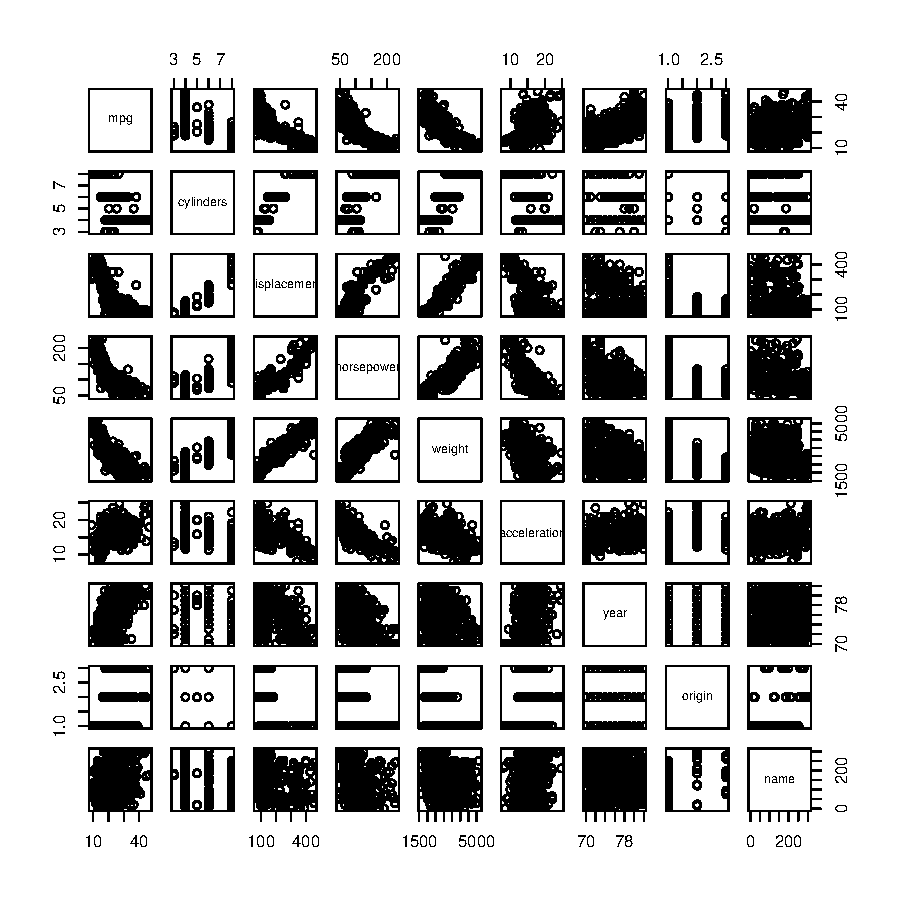
\includegraphics{mutivariblelm-9a}


\part{b}
\begin{Schunk}
\begin{Sinput}
> cor(auto[, -9])
\end{Sinput}
\begin{Soutput}
                    mpg  cylinders displacement horsepower     weight
mpg           1.0000000 -0.7776175   -0.8051269 -0.7784268 -0.8322442
cylinders    -0.7776175  1.0000000    0.9508233  0.8429834  0.8975273
displacement -0.8051269  0.9508233    1.0000000  0.8972570  0.9329944
horsepower   -0.7784268  0.8429834    0.8972570  1.0000000  0.8645377
weight       -0.8322442  0.8975273    0.9329944  0.8645377  1.0000000
acceleration  0.4233285 -0.5046834   -0.5438005 -0.6891955 -0.4168392
year          0.5805410 -0.3456474   -0.3698552 -0.4163615 -0.3091199
origin        0.5652088 -0.5689316   -0.6145351 -0.4551715 -0.5850054
             acceleration       year     origin
mpg             0.4233285  0.5805410  0.5652088
cylinders      -0.5046834 -0.3456474 -0.5689316
displacement   -0.5438005 -0.3698552 -0.6145351
horsepower     -0.6891955 -0.4163615 -0.4551715
weight         -0.4168392 -0.3091199 -0.5850054
acceleration    1.0000000  0.2903161  0.2127458
year            0.2903161  1.0000000  0.1815277
origin          0.2127458  0.1815277  1.0000000
\end{Soutput}
\end{Schunk}


\part{c}
\begin{Schunk}
\begin{Sinput}
> fit1 = lm(mpg ~ cylinders + displacement + horsepower + weight + acceleration + year + origin)
> summary(fit1)
\end{Sinput}
\begin{Soutput}
Call:
lm(formula = mpg ~ cylinders + displacement + horsepower + weight + 
    acceleration + year + origin)

Residuals:
    Min      1Q  Median      3Q     Max 
-9.5903 -2.1565 -0.1169  1.8690 13.0604 

Coefficients:
               Estimate Std. Error t value Pr(>|t|)    
(Intercept)  -17.218435   4.644294  -3.707  0.00024 ***
cylinders     -0.493376   0.323282  -1.526  0.12780    
displacement   0.019896   0.007515   2.647  0.00844 ** 
horsepower    -0.016951   0.013787  -1.230  0.21963    
weight        -0.006474   0.000652  -9.929  < 2e-16 ***
acceleration   0.080576   0.098845   0.815  0.41548    
year           0.750773   0.050973  14.729  < 2e-16 ***
origin         1.426141   0.278136   5.127 4.67e-07 ***
---
Signif. codes:  0 ‘***’ 0.001 ‘**’ 0.01 ‘*’ 0.05 ‘.’ 0.1 ‘ ’ 1

Residual standard error: 3.328 on 384 degrees of freedom
Multiple R-squared:  0.8215,	Adjusted R-squared:  0.8182 
F-statistic: 252.4 on 7 and 384 DF,  p-value: < 2.2e-16
\end{Soutput}
\end{Schunk}
\begin{enumerate}
{\color{red}
\item As we can see from the summary, the p-value for many preditors are very small, and the F-statistic is much bigger than 1. So, there is a relationship between the predictor and the response.

\item As we can see that the the p-value for displacement, weight, year and origin is very small which means these 4 preditors have significant relationship the response while cylinders, horsepower and acceleration not.

\item The coeffcient of year means that with time goes on, cars are more energy efficient. Cars can travel more miles with the same amount of gas.
}
\end{enumerate}

\part{d}
\begin{Schunk}
\begin{Sinput}
> par(mfrow = c(2, 2))
> plot(fit1)
\end{Sinput}
\end{Schunk}
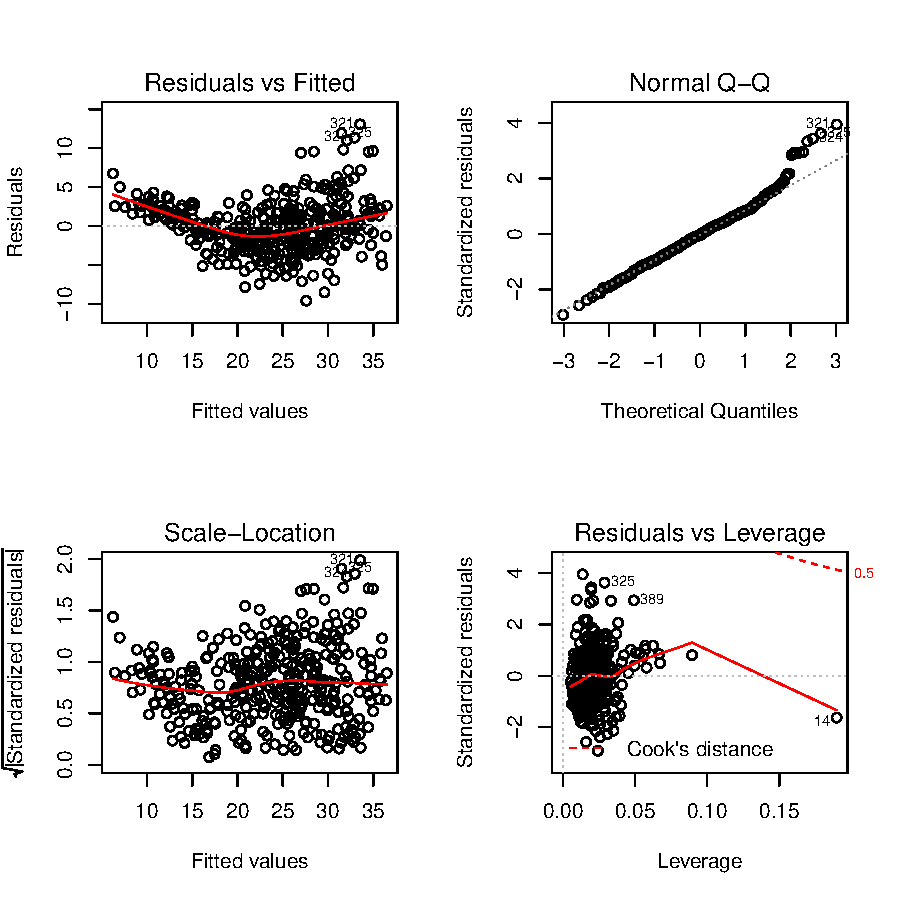
\includegraphics{mutivariblelm-9d}
\begin{enumerate}
{\color{red}
\item The plot of residuals shows that this linear model is not a good fit of the data. first we can see that the residuals are not uniformly spread along the h = 0 line, which is not a Gussian distribution.
\item We can see some large outliers in the plot which are data points 321, 324 and 325.
\item The point 14 has a unusually high leverage
}
\end{enumerate}


\part{e}
\begin{Schunk}
\begin{Sinput}
> fit2 = lm(mpg ~ displacement * weight   + year * origin)
> summary(fit2)
\end{Sinput}
\begin{Soutput}
Call:
lm(formula = mpg ~ displacement * weight + year * origin)

Residuals:
    Min      1Q  Median      3Q     Max 
-9.5758 -1.6211 -0.0537  1.3264 13.3266 

Coefficients:
                      Estimate Std. Error t value Pr(>|t|)    
(Intercept)          1.793e+01  8.044e+00   2.229 0.026394 *  
displacement        -7.519e-02  9.091e-03  -8.271 2.19e-15 ***
weight              -1.035e-02  6.450e-04 -16.053  < 2e-16 ***
year                 4.864e-01  1.017e-01   4.782 2.47e-06 ***
origin              -1.503e+01  4.232e+00  -3.551 0.000432 ***
displacement:weight  2.098e-05  2.179e-06   9.625  < 2e-16 ***
year:origin          1.980e-01  5.436e-02   3.642 0.000308 ***
---
Signif. codes:  0 ‘***’ 0.001 ‘**’ 0.01 ‘*’ 0.05 ‘.’ 0.1 ‘ ’ 1

Residual standard error: 2.969 on 385 degrees of freedom
Multiple R-squared:  0.8575,	Adjusted R-squared:  0.8553 
F-statistic: 386.2 on 6 and 385 DF,  p-value: < 2.2e-16
\end{Soutput}
\begin{Sinput}
> par(mfrow = c(2,2))
> plot(fit2)
\end{Sinput}
\end{Schunk}
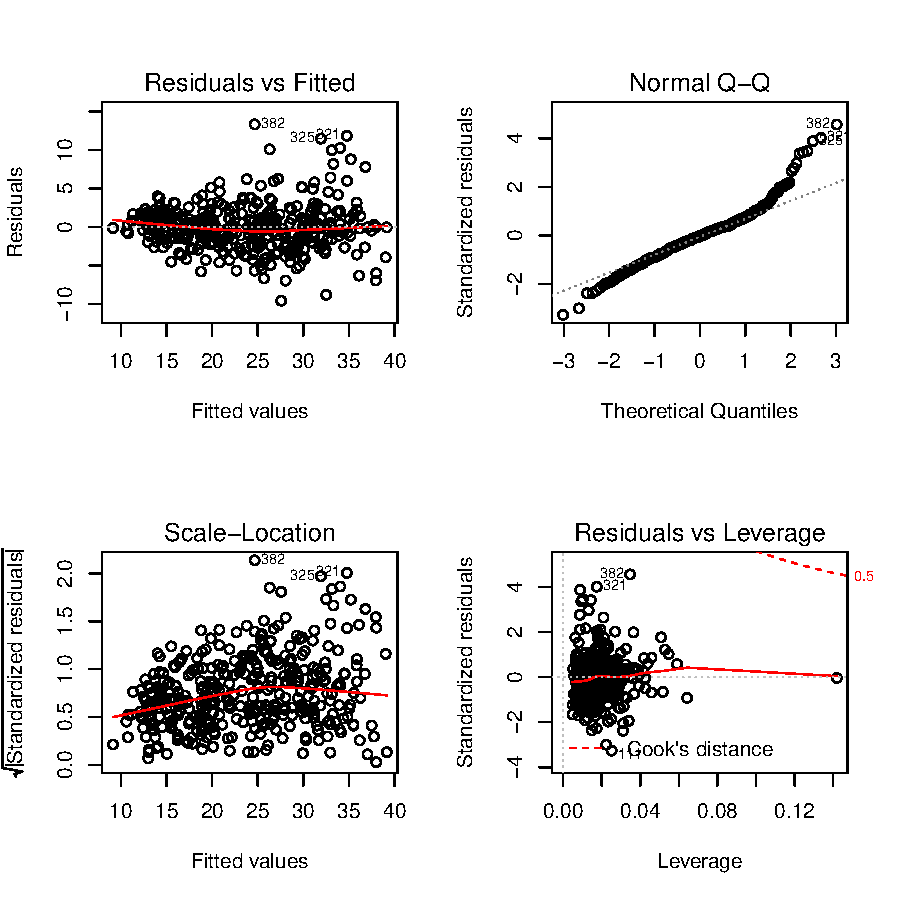
\includegraphics{mutivariblelm-9e}
\begin{enumerate}
{\color{red}
\item The interaction between displacement and weight appear to be statistically significant.
}
\end{enumerate}

\part{f}
\begin{Schunk}
\begin{Sinput}
> fit3 = lm(mpg ~ sqrt(displacement) + sqrt(weight) + log(displacement * weight)   + sqrt(acceleration) + year)
> summary(fit3)
\end{Sinput}
\begin{Soutput}
Call:
lm(formula = mpg ~ sqrt(displacement) + sqrt(weight) + log(displacement * 
    weight) + sqrt(acceleration) + year)

Residuals:
     Min       1Q   Median       3Q      Max 
-11.2912  -1.7534  -0.0111   1.6147  12.3624 

Coefficients:
                           Estimate Std. Error t value Pr(>|t|)    
(Intercept)                163.9452    20.4053   8.034 1.15e-14 ***
sqrt(displacement)           2.5693     0.3620   7.098 6.12e-12 ***
sqrt(weight)                 0.0310     0.1105   0.281   0.7791    
log(displacement * weight) -18.5851     2.3277  -7.984 1.64e-14 ***
sqrt(acceleration)           1.0258     0.5581   1.838   0.0668 .  
year                         0.8218     0.0459  17.903  < 2e-16 ***
---
Signif. codes:  0 ‘***’ 0.001 ‘**’ 0.01 ‘*’ 0.05 ‘.’ 0.1 ‘ ’ 1

Residual standard error: 3.041 on 386 degrees of freedom
Multiple R-squared:  0.8501,	Adjusted R-squared:  0.8482 
F-statistic: 437.8 on 5 and 386 DF,  p-value: < 2.2e-16
\end{Soutput}
\begin{Sinput}
> par(mfrow = c(2,2))
> plot(fit3)
\end{Sinput}
\end{Schunk}
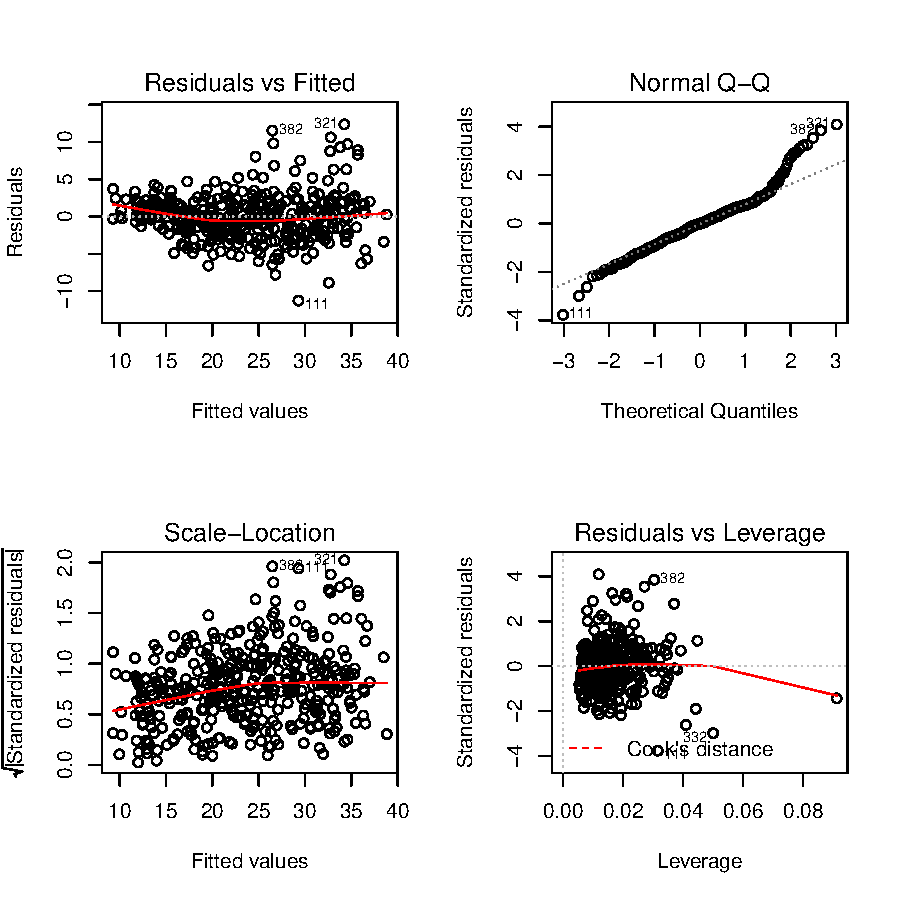
\includegraphics{mutivariblelm-9f1}

\begin{enumerate}
{\color{red}
\item From the residual plot, we can see that this model fit the data much better. The red line is almost flat compared with the gray line h = 0; But at begining, the red line still lie above the gray line.
\item There are still some outliers. But compared with initail fit, these outliers are less diviated from the mean of standardlized residuals.
}
\end{enumerate}


\question{13}{linear regression}
\part{a}
\begin{Schunk}
\begin{Sinput}
> rm(list = ls())
> set.seed(1)
> X = rnorm(100)
\end{Sinput}
\end{Schunk}

\part{b}
\begin{Schunk}
\begin{Sinput}
> eps = rnorm(100, mean = 0, sd = sqrt(0.25))
\end{Sinput}
\end{Schunk}

\part{c}
\begin{Schunk}
\begin{Sinput}
> Y = -1 + 0.5 * X + eps
\end{Sinput}
\end{Schunk}
\begin{enumerate}
{\color{red}
\item The length of Y is 100
\item $\beta_0 = -1$, $\beta_1 = 0.5$
}
\end{enumerate}


\part{d}
\begin{Schunk}
\begin{Sinput}
> plot(X, Y)
\end{Sinput}
\end{Schunk}
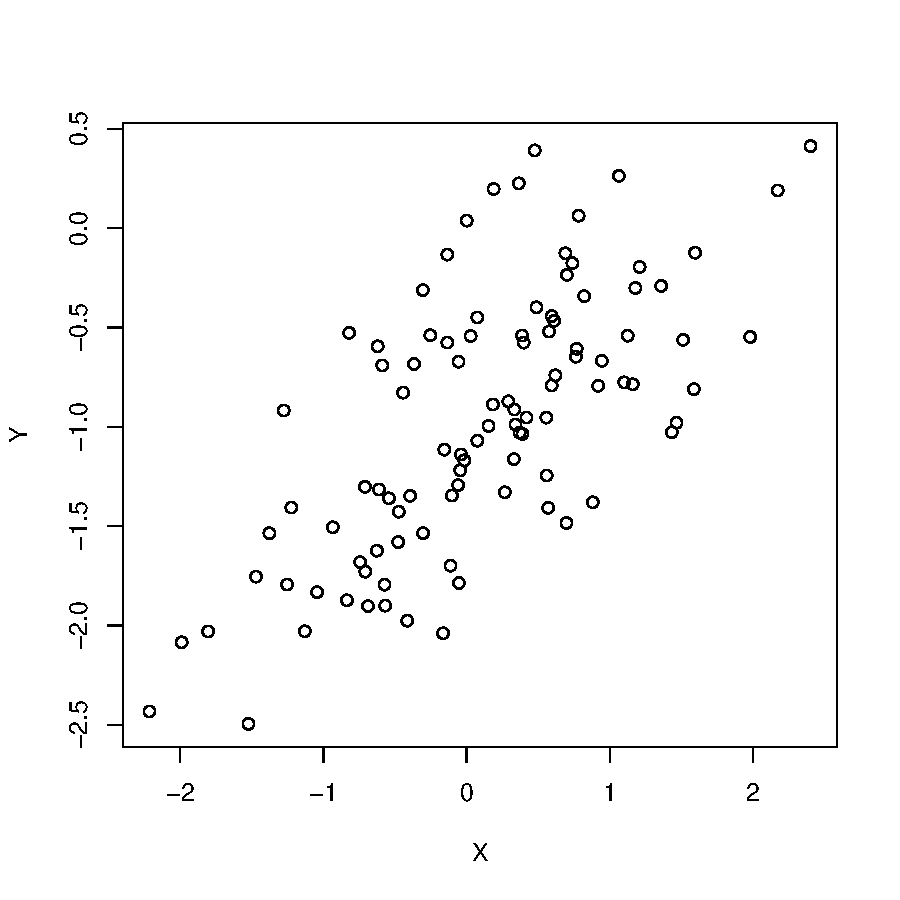
\includegraphics{mutivariblelm-13d}
\begin{enumerate}
{\color{red}
\item It seems that X and Y has a linear relationship.
}
\end{enumerate}


\part{e}
\begin{Schunk}
\begin{Sinput}
> fit.medium.noise = lm(Y ~ X)
> summary(fit.medium.noise)
\end{Sinput}
\begin{Soutput}
Call:
lm(formula = Y ~ X)

Residuals:
     Min       1Q   Median       3Q      Max 
-0.93842 -0.30688 -0.06975  0.26970  1.17309 

Coefficients:
            Estimate Std. Error t value Pr(>|t|)    
(Intercept) -1.01885    0.04849 -21.010  < 2e-16 ***
X            0.49947    0.05386   9.273 4.58e-15 ***
---
Signif. codes:  0 ‘***’ 0.001 ‘**’ 0.01 ‘*’ 0.05 ‘.’ 0.1 ‘ ’ 1

Residual standard error: 0.4814 on 98 degrees of freedom
Multiple R-squared:  0.4674,	Adjusted R-squared:  0.4619 
F-statistic: 85.99 on 1 and 98 DF,  p-value: 4.583e-15
\end{Soutput}
\end{Schunk}
\begin{enumerate}
{\color{red}
\item $\hat{beta_0} = -1.01885$, $\hat{beta_1} = 0.49947$, both are very close to the original value.
}
\end{enumerate}

\part{f}
\begin{Schunk}
\begin{Sinput}
> plot(X, Y)
> abline(-1, 0.5, col = 2)
> abline(fit.medium.noise, col = 3)
> legend(x = 1.2, y = -1.5, legend = c("original", "fit"), col = 2:3, lwd = 1)
\end{Sinput}
\end{Schunk}


\part{g}
\begin{Schunk}
\begin{Sinput}
> fit = lm(Y ~ X + I(X ^ 2))
> summary(fit)
\end{Sinput}
\begin{Soutput}
Call:
lm(formula = Y ~ X + I(X^2))

Residuals:
     Min       1Q   Median       3Q      Max 
-0.98252 -0.31270 -0.06441  0.29014  1.13500 

Coefficients:
            Estimate Std. Error t value Pr(>|t|)    
(Intercept) -0.97164    0.05883 -16.517  < 2e-16 ***
X            0.50858    0.05399   9.420  2.4e-15 ***
I(X^2)      -0.05946    0.04238  -1.403    0.164    
---
Signif. codes:  0 ‘***’ 0.001 ‘**’ 0.01 ‘*’ 0.05 ‘.’ 0.1 ‘ ’ 1

Residual standard error: 0.479 on 97 degrees of freedom
Multiple R-squared:  0.4779,	Adjusted R-squared:  0.4672 
F-statistic:  44.4 on 2 and 97 DF,  p-value: 2.038e-14
\end{Soutput}
\end{Schunk}
\begin{enumerate}
{\color{red}
\item The p-value of the quadratic term is 0.852, which means there's no relationship between the quadratic term and Y.
}
\end{enumerate}

\part{h}
\begin{Schunk}
\begin{Sinput}
> set.seed(1)
> X = rnorm(100)
> eps = rnorm(100, mean = 0, sd = sqrt(0.1))
> Y = -1 + 0.5 * X + eps
> fit.less.noise = lm(Y ~ X)
> summary(fit.less.noise)
\end{Sinput}
\begin{Soutput}
Call:
lm(formula = Y ~ X)

Residuals:
     Min       1Q   Median       3Q      Max 
-0.59351 -0.19409 -0.04411  0.17057  0.74193 

Coefficients:
            Estimate Std. Error t value Pr(>|t|)    
(Intercept) -1.01192    0.03067  -32.99   <2e-16 ***
X            0.49966    0.03407   14.67   <2e-16 ***
---
Signif. codes:  0 ‘***’ 0.001 ‘**’ 0.01 ‘*’ 0.05 ‘.’ 0.1 ‘ ’ 1

Residual standard error: 0.3044 on 98 degrees of freedom
Multiple R-squared:  0.687,	Adjusted R-squared:  0.6838 
F-statistic: 215.1 on 1 and 98 DF,  p-value: < 2.2e-16
\end{Soutput}
\begin{Sinput}
> plot(X, Y)
> abline(-1, 0.5, col = 1)
> abline(fit.less.noise, col = 2)
> legend(x = 1.2, y = -1.5, legend = c("original", "fit"), col = 1:2, lwd = 1)
\end{Sinput}
\end{Schunk}
\begin{enumerate}
{\color{red}
\item After decreasing the noise of eps, the linear model fit the original model very well. $\hat{\beta_0} = -1.01192$ and $\hat{\beta_1} = 0.49966$, both of which are much closer to the original value but not better.
\item The decreasing of noise does not influence $\hat{\beta_0}$ and $\hat{\beta_1}$ too much.
\item $R^2$ increased
}
\end{enumerate}


\part{i}
\begin{Schunk}
\begin{Sinput}
> set.seed(1)
> X = rnorm(100)
> eps = rnorm(100, mean = 0, sd = sqrt(0.5))
> Y = -1 + 0.5 * X + eps
> fit.more.noise = lm(Y ~ X)
> summary(fit.more.noise)
\end{Sinput}
\begin{Soutput}
Call:
lm(formula = Y ~ X)

Residuals:
     Min       1Q   Median       3Q      Max 
-1.32713 -0.43400 -0.09864  0.38141  1.65900 

Coefficients:
            Estimate Std. Error t value Pr(>|t|)    
(Intercept) -1.02665    0.06858 -14.970  < 2e-16 ***
X            0.49925    0.07617   6.554 2.62e-09 ***
---
Signif. codes:  0 ‘***’ 0.001 ‘**’ 0.01 ‘*’ 0.05 ‘.’ 0.1 ‘ ’ 1

Residual standard error: 0.6808 on 98 degrees of freedom
Multiple R-squared:  0.3047,	Adjusted R-squared:  0.2976 
F-statistic: 42.96 on 1 and 98 DF,  p-value: 2.624e-09
\end{Soutput}
\begin{Sinput}
> plot(X, Y)
> abline(-1, 0.5, col = 1)
> abline(fit.more.noise, col = 2)
> legend(x = 1.2, y = -1.5, legend = c("original", "fit"), col = 1:2, lwd = 1)
\end{Sinput}
\end{Schunk}
\begin{enumerate}
{\color{red}
\item After decreasing the noise of eps, the linear model fit the original model very well. $\hat{\beta_0} = -1.02665$ and $\hat{\beta_1} = 0.49925$, both of which are much closer to the original value but not better.
\item The decreasing of noise does not influence $\hat{\beta_0}$ and $\hat{\beta_1}$ too much.
\item $R^2$ decreased.
}
\end{enumerate}


\part{j}
\begin{Schunk}
\begin{Sinput}
> confint(fit.medium.noise)
\end{Sinput}
\begin{Soutput}
                 2.5 %     97.5 %
(Intercept) -1.1150804 -0.9226122
X            0.3925794  0.6063602
\end{Soutput}
\begin{Sinput}
> confint(fit.less.noise)
\end{Sinput}
\begin{Soutput}
                 2.5 %     97.5 %
(Intercept) -1.0727832 -0.9510557
X            0.4320613  0.5672681
\end{Soutput}
\begin{Sinput}
> confint(fit.more.noise)
\end{Sinput}
\begin{Soutput}
                 2.5 %     97.5 %
(Intercept) -1.1627482 -0.8905572
X            0.3480843  0.6504160
\end{Soutput}
\end{Schunk}
\begin{enumerate}
{\color{red}
\item It's easy to see that with less noise, the confident interval tend to be narrower and with more noise, the confident interval tend to be wider.
}
\end{enumerate}


\question{15}{Boston Crime Rate}
\part{a}
\begin{Schunk}
\begin{Sinput}
> rm(list = ls())
> library(MASS)
> attach(Boston)
> fit.age = lm(crim ~ age)
> summary(fit.age)
\end{Sinput}
\begin{Soutput}
Call:
lm(formula = crim ~ age)

Residuals:
   Min     1Q Median     3Q    Max 
-6.789 -4.257 -1.230  1.527 82.849 

Coefficients:
            Estimate Std. Error t value Pr(>|t|)    
(Intercept) -3.77791    0.94398  -4.002 7.22e-05 ***
age          0.10779    0.01274   8.463 2.85e-16 ***
---
Signif. codes:  0 ‘***’ 0.001 ‘**’ 0.01 ‘*’ 0.05 ‘.’ 0.1 ‘ ’ 1

Residual standard error: 8.057 on 504 degrees of freedom
Multiple R-squared:  0.1244,	Adjusted R-squared:  0.1227 
F-statistic: 71.62 on 1 and 504 DF,  p-value: 2.855e-16
\end{Soutput}
\begin{Sinput}
> par(mfrow = c(2,2))
> plot(fit.age)
\end{Sinput}
\end{Schunk}
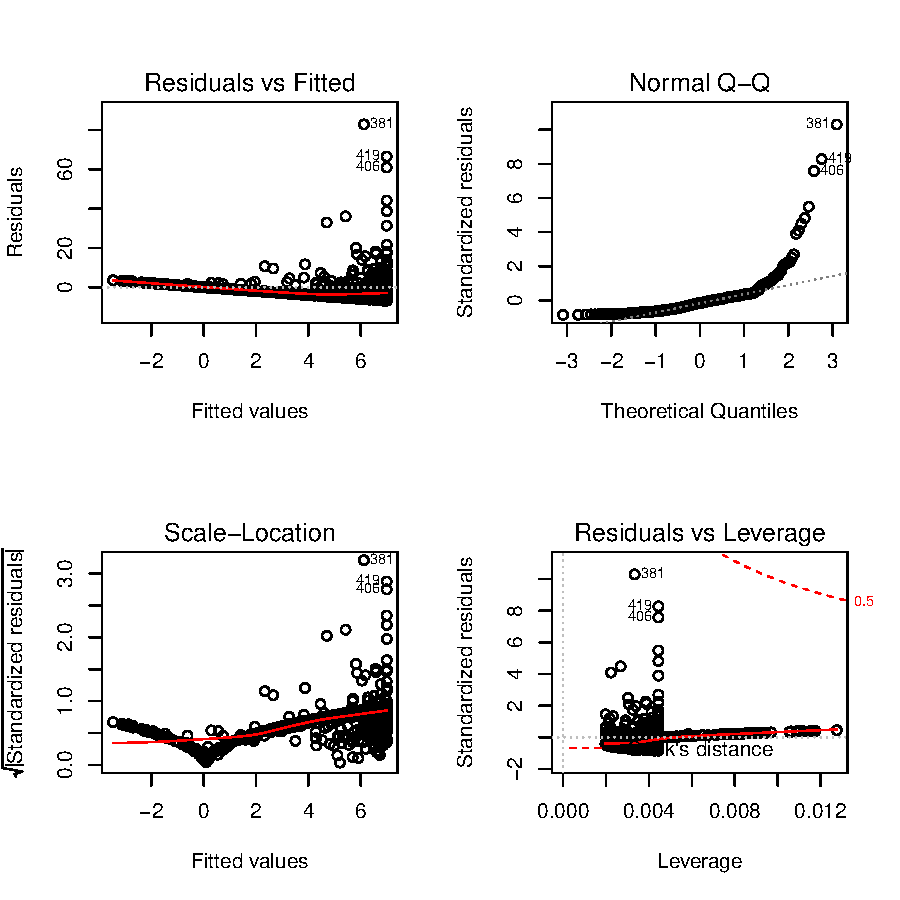
\includegraphics{mutivariblelm-age}

\begin{Schunk}
\begin{Sinput}
> fit.black = lm(crim ~ black)
> summary(fit.black)
\end{Sinput}
\begin{Soutput}
Call:
lm(formula = crim ~ black)

Residuals:
    Min      1Q  Median      3Q     Max 
-13.756  -2.299  -2.095  -1.296  86.822 

Coefficients:
             Estimate Std. Error t value Pr(>|t|)    
(Intercept) 16.553529   1.425903  11.609   <2e-16 ***
black       -0.036280   0.003873  -9.367   <2e-16 ***
---
Signif. codes:  0 ‘***’ 0.001 ‘**’ 0.01 ‘*’ 0.05 ‘.’ 0.1 ‘ ’ 1

Residual standard error: 7.946 on 504 degrees of freedom
Multiple R-squared:  0.1483,	Adjusted R-squared:  0.1466 
F-statistic: 87.74 on 1 and 504 DF,  p-value: < 2.2e-16
\end{Soutput}
\begin{Sinput}
> par(mfrow = c(2,2))
> plot(fit.black)
\end{Sinput}
\end{Schunk}
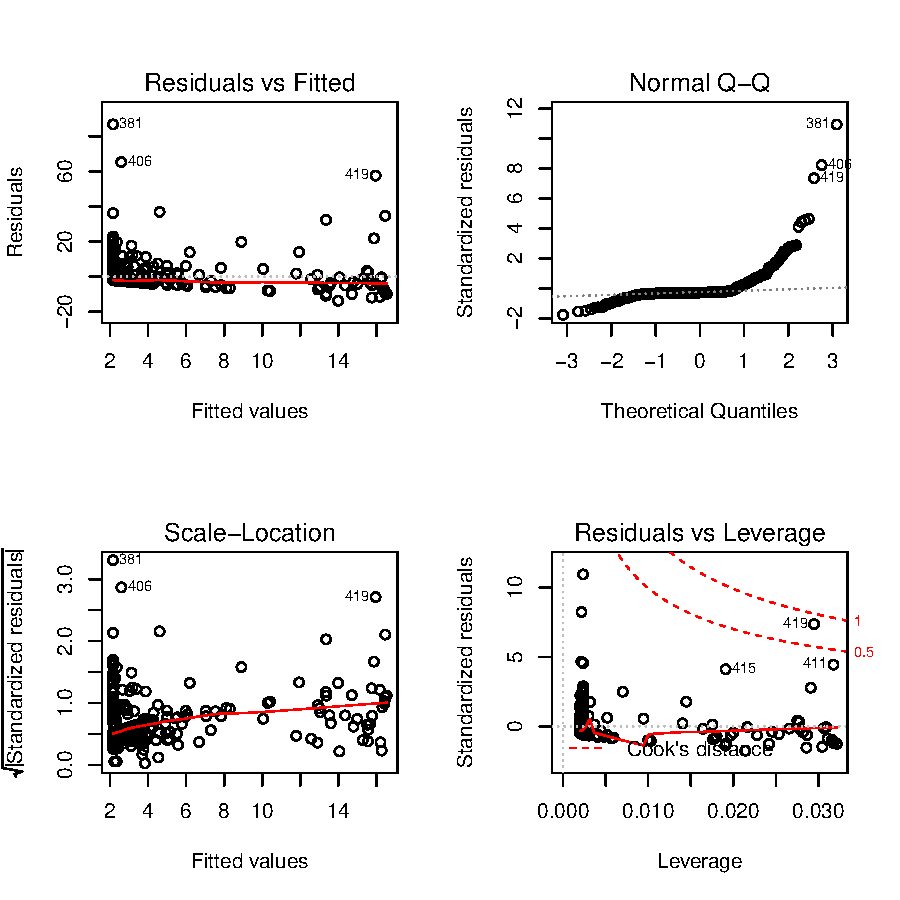
\includegraphics{mutivariblelm-black}


\begin{Schunk}
\begin{Sinput}
> fit.chas = lm(crim ~ chas)
> summary(fit.chas)
\end{Sinput}
\begin{Soutput}
Call:
lm(formula = crim ~ chas)

Residuals:
   Min     1Q Median     3Q    Max 
-3.738 -3.661 -3.435  0.018 85.232 

Coefficients:
            Estimate Std. Error t value Pr(>|t|)    
(Intercept)   3.7444     0.3961   9.453   <2e-16 ***
chas         -1.8928     1.5061  -1.257    0.209    
---
Signif. codes:  0 ‘***’ 0.001 ‘**’ 0.01 ‘*’ 0.05 ‘.’ 0.1 ‘ ’ 1

Residual standard error: 8.597 on 504 degrees of freedom
Multiple R-squared:  0.003124,	Adjusted R-squared:  0.001146 
F-statistic: 1.579 on 1 and 504 DF,  p-value: 0.2094
\end{Soutput}
\begin{Sinput}
> par(mfrow = c(2,2))
> plot(fit.chas)
\end{Sinput}
\end{Schunk}
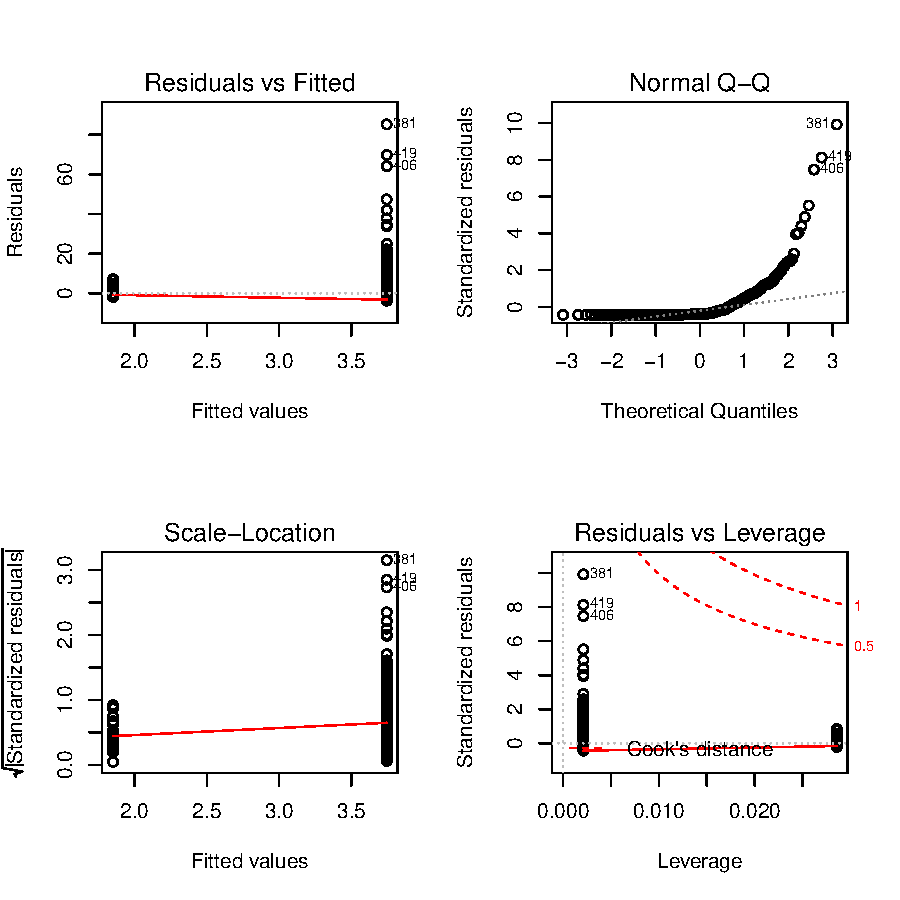
\includegraphics{mutivariblelm-chas}

\begin{Schunk}
\begin{Sinput}
> fit.dis = lm(crim ~ dis)
> summary(fit.dis)
\end{Sinput}
\begin{Soutput}
Call:
lm(formula = crim ~ dis)

Residuals:
   Min     1Q Median     3Q    Max 
-6.708 -4.134 -1.527  1.516 81.674 

Coefficients:
            Estimate Std. Error t value Pr(>|t|)    
(Intercept)   9.4993     0.7304  13.006   <2e-16 ***
dis          -1.5509     0.1683  -9.213   <2e-16 ***
---
Signif. codes:  0 ‘***’ 0.001 ‘**’ 0.01 ‘*’ 0.05 ‘.’ 0.1 ‘ ’ 1

Residual standard error: 7.965 on 504 degrees of freedom
Multiple R-squared:  0.1441,	Adjusted R-squared:  0.1425 
F-statistic: 84.89 on 1 and 504 DF,  p-value: < 2.2e-16
\end{Soutput}
\begin{Sinput}
> par(mfrow = c(2,2))
> plot(fit.dis)
\end{Sinput}
\end{Schunk}
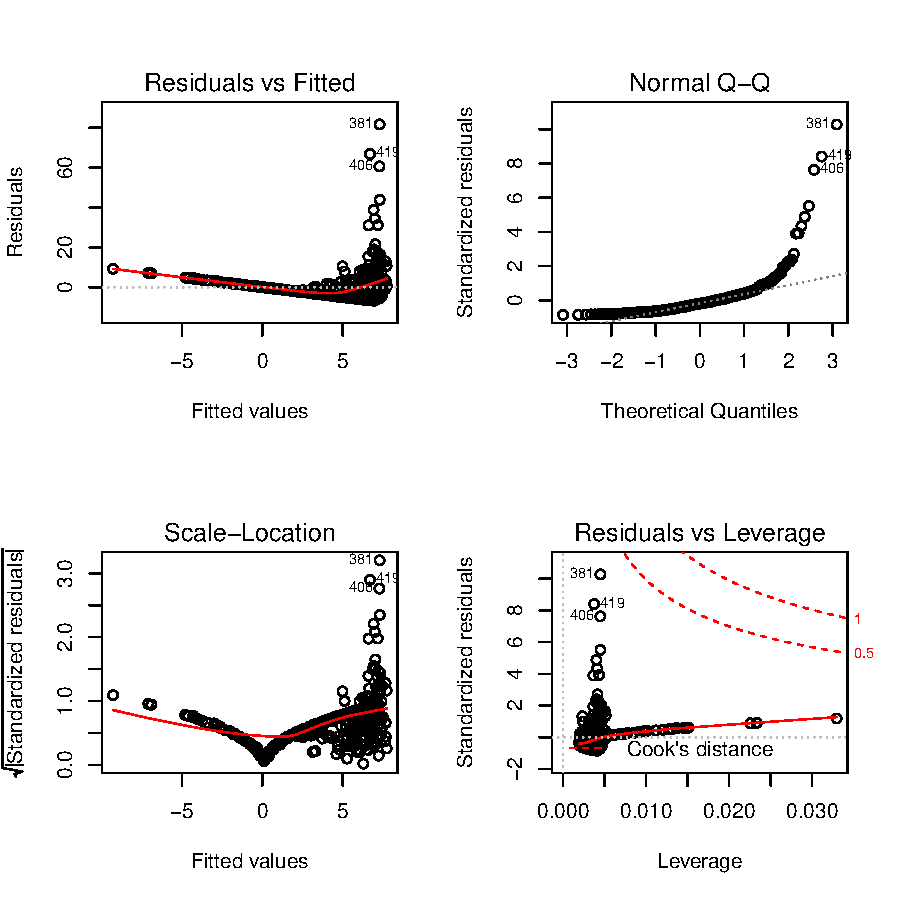
\includegraphics{mutivariblelm-dis}

\begin{Schunk}
\begin{Sinput}
> fit.indus = lm(crim ~ indus)
> summary(fit.indus)
\end{Sinput}
\begin{Soutput}
Call:
lm(formula = crim ~ indus)

Residuals:
    Min      1Q  Median      3Q     Max 
-11.972  -2.698  -0.736   0.712  81.813 

Coefficients:
            Estimate Std. Error t value Pr(>|t|)    
(Intercept) -2.06374    0.66723  -3.093  0.00209 ** 
indus        0.50978    0.05102   9.991  < 2e-16 ***
---
Signif. codes:  0 ‘***’ 0.001 ‘**’ 0.01 ‘*’ 0.05 ‘.’ 0.1 ‘ ’ 1

Residual standard error: 7.866 on 504 degrees of freedom
Multiple R-squared:  0.1653,	Adjusted R-squared:  0.1637 
F-statistic: 99.82 on 1 and 504 DF,  p-value: < 2.2e-16
\end{Soutput}
\begin{Sinput}
> par(mfrow = c(2,2))
> plot(fit.indus)
\end{Sinput}
\end{Schunk}
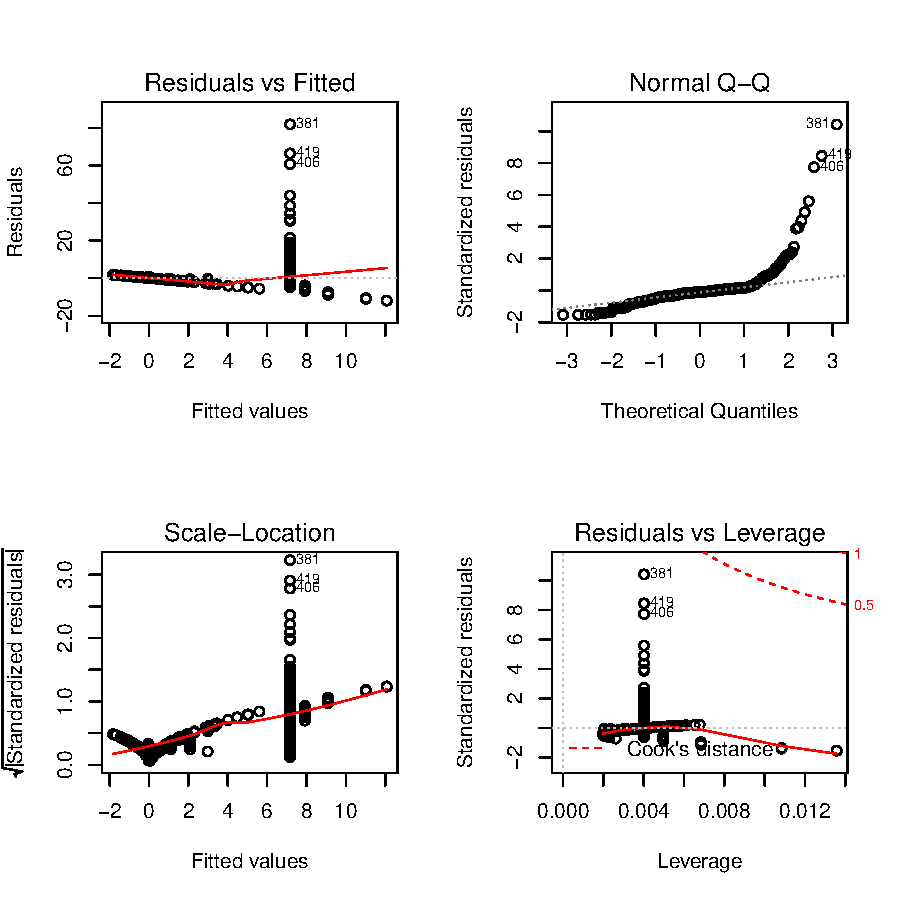
\includegraphics{mutivariblelm-indus}

\begin{Schunk}
\begin{Sinput}
> fit.lstat = lm(crim ~ lstat)
> summary(fit.lstat)
\end{Sinput}
\begin{Soutput}
Call:
lm(formula = crim ~ lstat)

Residuals:
    Min      1Q  Median      3Q     Max 
-13.925  -2.822  -0.664   1.079  82.862 

Coefficients:
            Estimate Std. Error t value Pr(>|t|)    
(Intercept) -3.33054    0.69376  -4.801 2.09e-06 ***
lstat        0.54880    0.04776  11.491  < 2e-16 ***
---
Signif. codes:  0 ‘***’ 0.001 ‘**’ 0.01 ‘*’ 0.05 ‘.’ 0.1 ‘ ’ 1

Residual standard error: 7.664 on 504 degrees of freedom
Multiple R-squared:  0.2076,	Adjusted R-squared:  0.206 
F-statistic:   132 on 1 and 504 DF,  p-value: < 2.2e-16
\end{Soutput}
\begin{Sinput}
> par(mfrow = c(2,2))
> plot(fit.lstat)
\end{Sinput}
\end{Schunk}
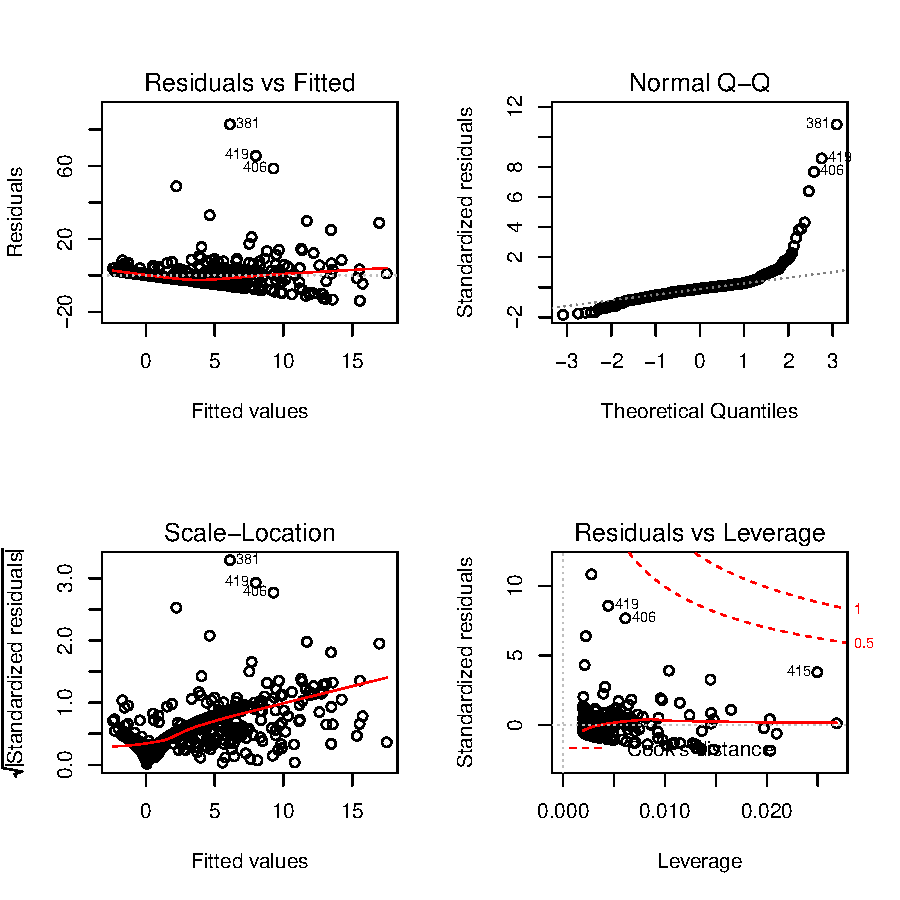
\includegraphics{mutivariblelm-lstat}

\begin{Schunk}
\begin{Sinput}
> fit.medv = lm(crim ~ medv)
> summary(fit.medv)
\end{Sinput}
\begin{Soutput}
Call:
lm(formula = crim ~ medv)

Residuals:
   Min     1Q Median     3Q    Max 
-9.071 -4.022 -2.343  1.298 80.957 

Coefficients:
            Estimate Std. Error t value Pr(>|t|)    
(Intercept) 11.79654    0.93419   12.63   <2e-16 ***
medv        -0.36316    0.03839   -9.46   <2e-16 ***
---
Signif. codes:  0 ‘***’ 0.001 ‘**’ 0.01 ‘*’ 0.05 ‘.’ 0.1 ‘ ’ 1

Residual standard error: 7.934 on 504 degrees of freedom
Multiple R-squared:  0.1508,	Adjusted R-squared:  0.1491 
F-statistic: 89.49 on 1 and 504 DF,  p-value: < 2.2e-16
\end{Soutput}
\begin{Sinput}
> par(mfrow = c(2,2))
> plot(fit.medv)
\end{Sinput}
\end{Schunk}
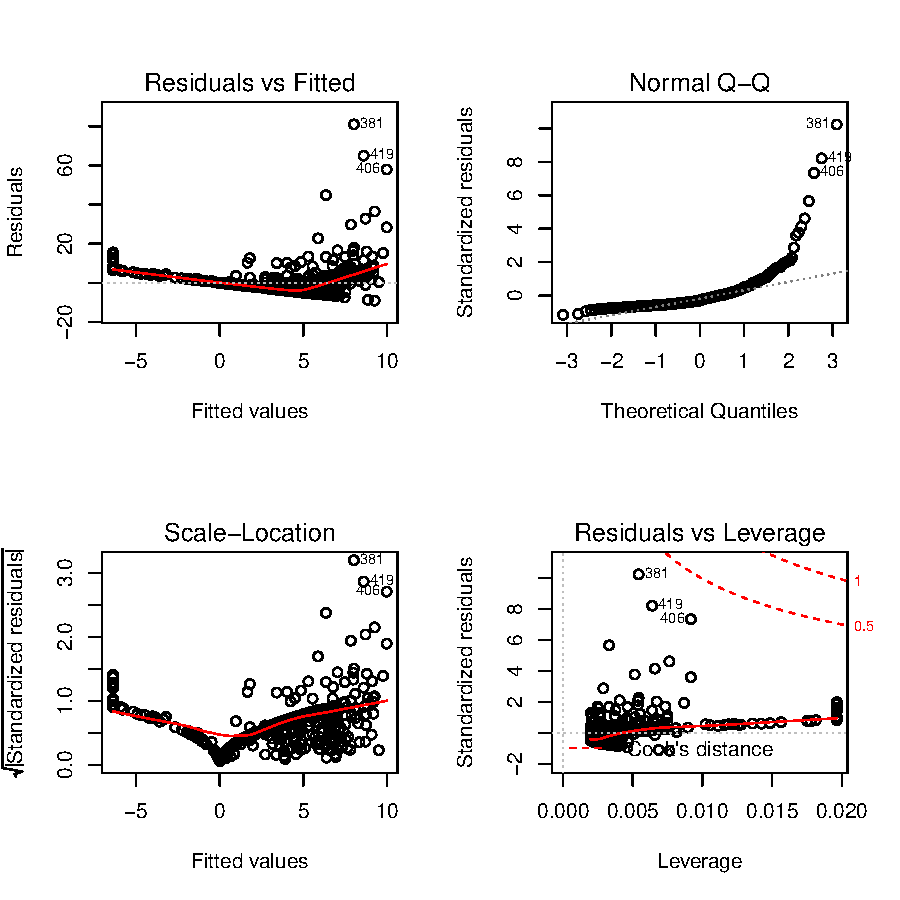
\includegraphics{mutivariblelm-medv}

\begin{Schunk}
\begin{Sinput}
> fit.nox = lm(crim ~ nox)
> summary(fit.nox)
\end{Sinput}
\begin{Soutput}
Call:
lm(formula = crim ~ nox)

Residuals:
    Min      1Q  Median      3Q     Max 
-12.371  -2.738  -0.974   0.559  81.728 

Coefficients:
            Estimate Std. Error t value Pr(>|t|)    
(Intercept)  -13.720      1.699  -8.073 5.08e-15 ***
nox           31.249      2.999  10.419  < 2e-16 ***
---
Signif. codes:  0 ‘***’ 0.001 ‘**’ 0.01 ‘*’ 0.05 ‘.’ 0.1 ‘ ’ 1

Residual standard error: 7.81 on 504 degrees of freedom
Multiple R-squared:  0.1772,	Adjusted R-squared:  0.1756 
F-statistic: 108.6 on 1 and 504 DF,  p-value: < 2.2e-16
\end{Soutput}
\begin{Sinput}
> par(mfrow = c(2,2))
> plot(fit.nox)
\end{Sinput}
\end{Schunk}
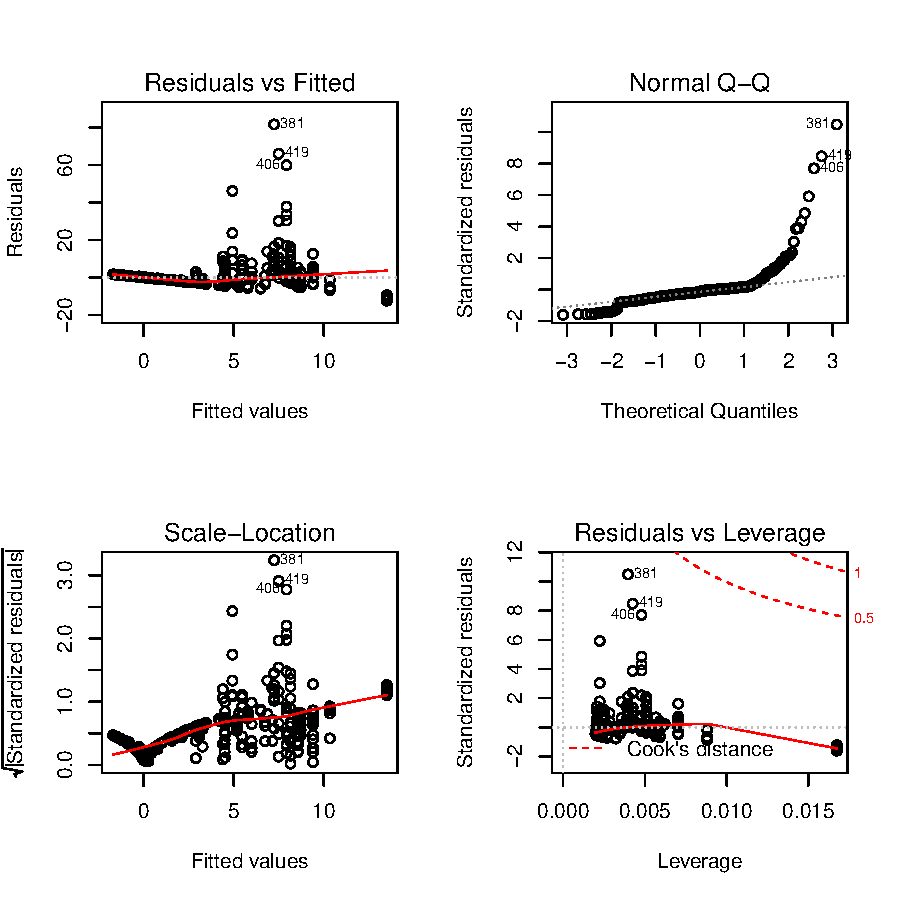
\includegraphics{mutivariblelm-nox}

\begin{Schunk}
\begin{Sinput}
> fit.ptratio = lm(crim ~ ptratio)
> summary(fit.ptratio)
\end{Sinput}
\begin{Soutput}
Call:
lm(formula = crim ~ ptratio)

Residuals:
   Min     1Q Median     3Q    Max 
-7.654 -3.985 -1.912  1.825 83.353 

Coefficients:
            Estimate Std. Error t value Pr(>|t|)    
(Intercept) -17.6469     3.1473  -5.607 3.40e-08 ***
ptratio       1.1520     0.1694   6.801 2.94e-11 ***
---
Signif. codes:  0 ‘***’ 0.001 ‘**’ 0.01 ‘*’ 0.05 ‘.’ 0.1 ‘ ’ 1

Residual standard error: 8.24 on 504 degrees of freedom
Multiple R-squared:  0.08407,	Adjusted R-squared:  0.08225 
F-statistic: 46.26 on 1 and 504 DF,  p-value: 2.943e-11
\end{Soutput}
\begin{Sinput}
> par(mfrow = c(2,2))
> plot(fit.ptratio)
\end{Sinput}
\end{Schunk}
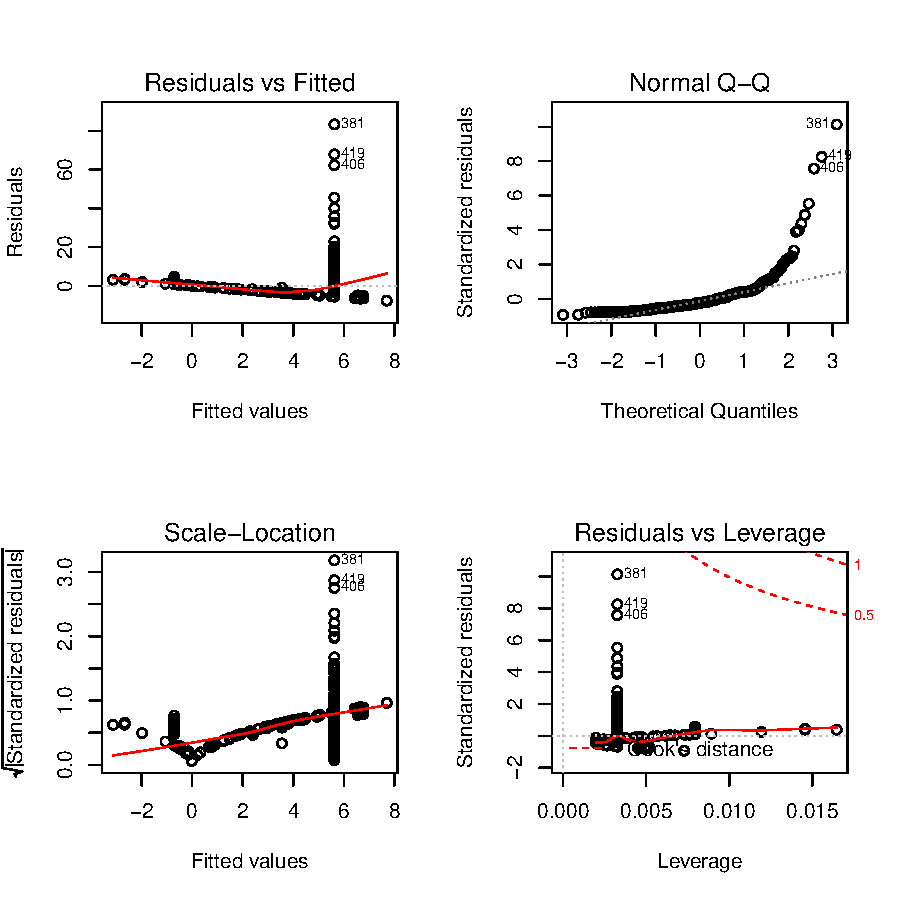
\includegraphics{mutivariblelm-ptratio}

\begin{Schunk}
\begin{Sinput}
> fit.rad = lm(crim ~ rad)
> summary(fit.rad)
\end{Sinput}
\begin{Soutput}
Call:
lm(formula = crim ~ rad)

Residuals:
    Min      1Q  Median      3Q     Max 
-10.164  -1.381  -0.141   0.660  76.433 

Coefficients:
            Estimate Std. Error t value Pr(>|t|)    
(Intercept) -2.28716    0.44348  -5.157 3.61e-07 ***
rad          0.61791    0.03433  17.998  < 2e-16 ***
---
Signif. codes:  0 ‘***’ 0.001 ‘**’ 0.01 ‘*’ 0.05 ‘.’ 0.1 ‘ ’ 1

Residual standard error: 6.718 on 504 degrees of freedom
Multiple R-squared:  0.3913,	Adjusted R-squared:   0.39 
F-statistic: 323.9 on 1 and 504 DF,  p-value: < 2.2e-16
\end{Soutput}
\begin{Sinput}
> par(mfrow = c(2,2))
> plot(fit.rad)
\end{Sinput}
\end{Schunk}
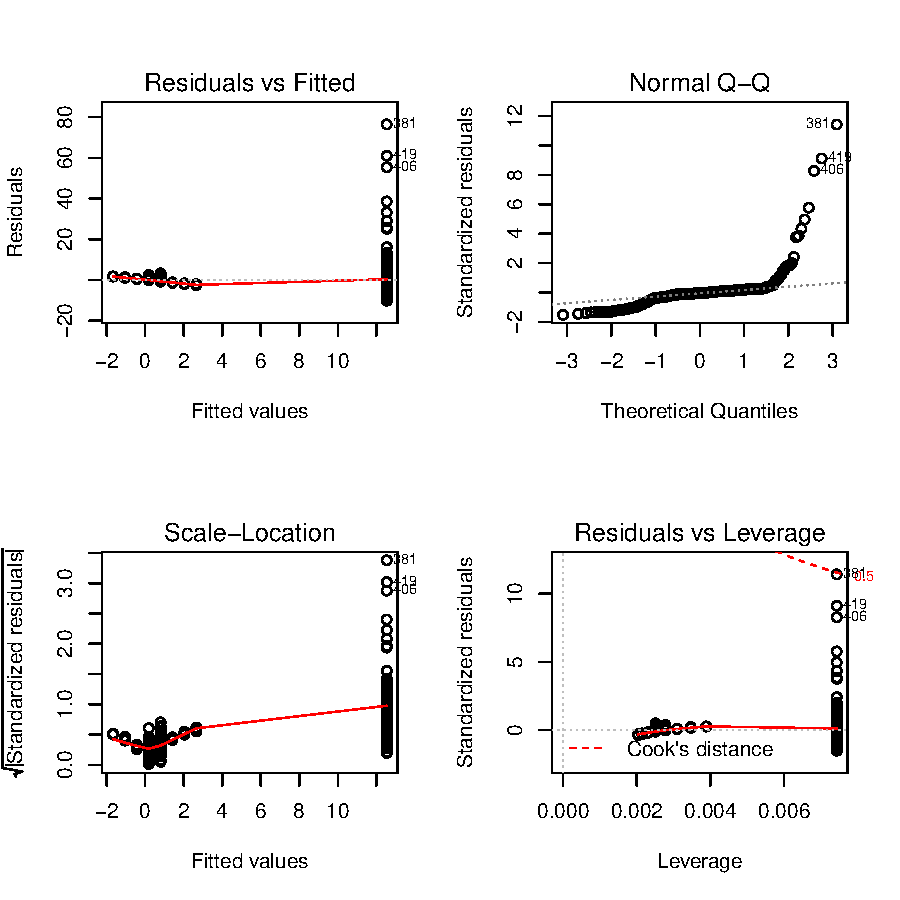
\includegraphics{mutivariblelm-rad}

\begin{Schunk}
\begin{Sinput}
> fit.rm = lm(crim ~ rm)
> summary(fit.rm)
\end{Sinput}
\begin{Soutput}
Call:
lm(formula = crim ~ rm)

Residuals:
   Min     1Q Median     3Q    Max 
-6.604 -3.952 -2.654  0.989 87.197 

Coefficients:
            Estimate Std. Error t value Pr(>|t|)    
(Intercept)   20.482      3.365   6.088 2.27e-09 ***
rm            -2.684      0.532  -5.045 6.35e-07 ***
---
Signif. codes:  0 ‘***’ 0.001 ‘**’ 0.01 ‘*’ 0.05 ‘.’ 0.1 ‘ ’ 1

Residual standard error: 8.401 on 504 degrees of freedom
Multiple R-squared:  0.04807,	Adjusted R-squared:  0.04618 
F-statistic: 25.45 on 1 and 504 DF,  p-value: 6.347e-07
\end{Soutput}
\begin{Sinput}
> par(mfrow = c(2,2))
> plot(fit.rm)
\end{Sinput}
\end{Schunk}
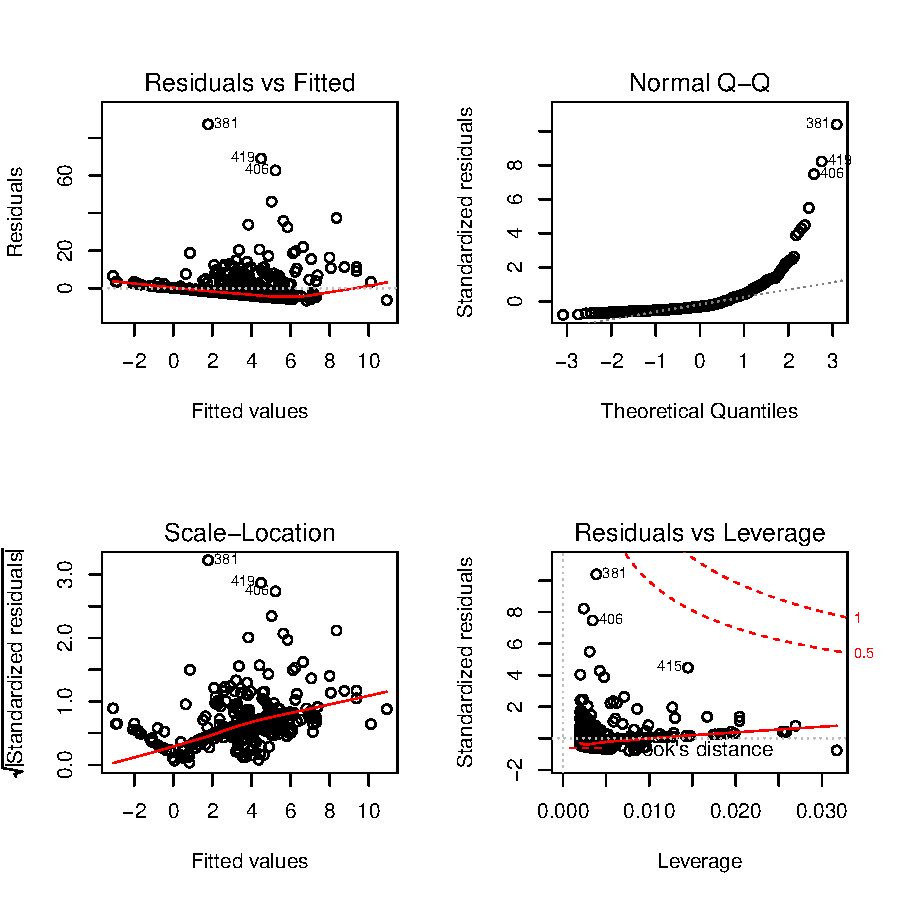
\includegraphics{mutivariblelm-rm}

\begin{Schunk}
\begin{Sinput}
> fit.tax = lm(crim ~ tax)
> summary(fit.tax)
\end{Sinput}
\begin{Soutput}
Call:
lm(formula = crim ~ tax)

Residuals:
    Min      1Q  Median      3Q     Max 
-12.513  -2.738  -0.194   1.065  77.696 

Coefficients:
             Estimate Std. Error t value Pr(>|t|)    
(Intercept) -8.528369   0.815809  -10.45   <2e-16 ***
tax          0.029742   0.001847   16.10   <2e-16 ***
---
Signif. codes:  0 ‘***’ 0.001 ‘**’ 0.01 ‘*’ 0.05 ‘.’ 0.1 ‘ ’ 1

Residual standard error: 6.997 on 504 degrees of freedom
Multiple R-squared:  0.3396,	Adjusted R-squared:  0.3383 
F-statistic: 259.2 on 1 and 504 DF,  p-value: < 2.2e-16
\end{Soutput}
\begin{Sinput}
> par(mfrow = c(2,2))
> plot(fit.tax)
\end{Sinput}
\end{Schunk}
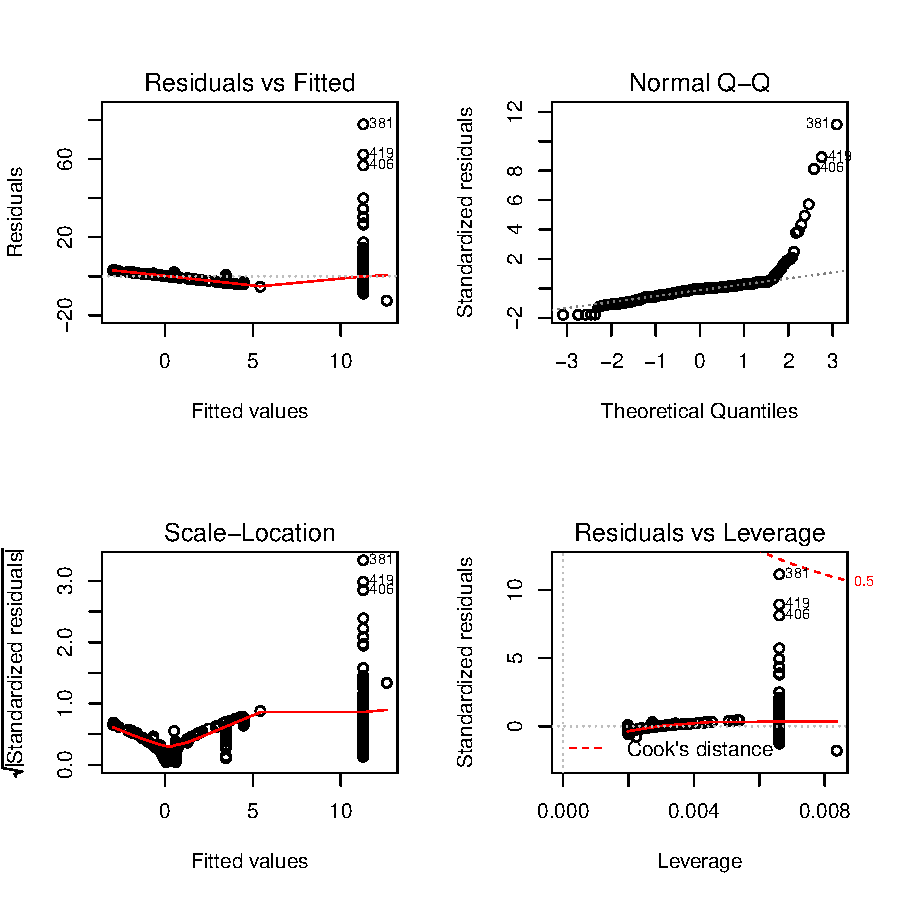
\includegraphics{mutivariblelm-tax}

\begin{Schunk}
\begin{Sinput}
> fit.zn = lm(crim ~ zn)
> summary(fit.zn)
\end{Sinput}
\begin{Soutput}
Call:
lm(formula = crim ~ zn)

Residuals:
   Min     1Q Median     3Q    Max 
-4.429 -4.222 -2.620  1.250 84.523 

Coefficients:
            Estimate Std. Error t value Pr(>|t|)    
(Intercept)  4.45369    0.41722  10.675  < 2e-16 ***
zn          -0.07393    0.01609  -4.594 5.51e-06 ***
---
Signif. codes:  0 ‘***’ 0.001 ‘**’ 0.01 ‘*’ 0.05 ‘.’ 0.1 ‘ ’ 1

Residual standard error: 8.435 on 504 degrees of freedom
Multiple R-squared:  0.04019,	Adjusted R-squared:  0.03828 
F-statistic:  21.1 on 1 and 504 DF,  p-value: 5.506e-06
\end{Soutput}
\begin{Sinput}
> par(mfrow = c(2,2))
> plot(fit.zn)
\end{Sinput}
\end{Schunk}
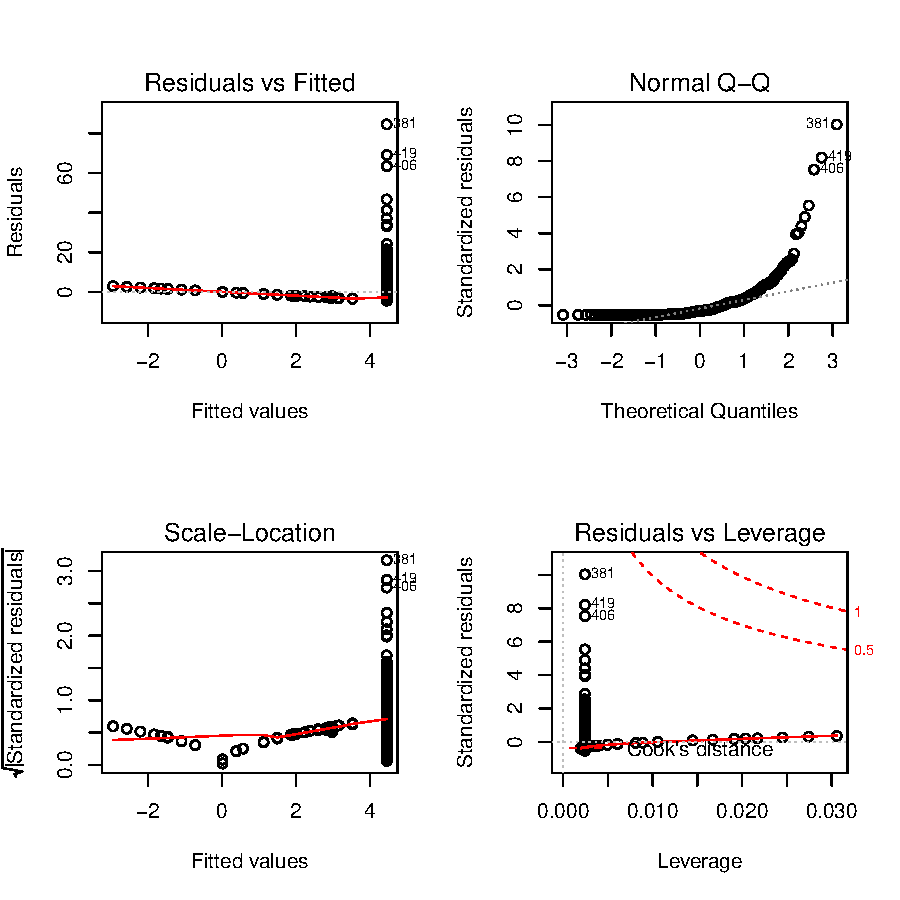
\includegraphics{mutivariblelm-zn}
\begin{enumerate}
{\color{red}
\item From those summaries and plots we can see that all the predictor except chas have statistically significant association with response crim.
}
\end{enumerate}


\part{b}
\begin{Schunk}
\begin{Sinput}
> fit.all = lm(crim ~ ., data = Boston)
> summary(fit.all)
\end{Sinput}
\begin{Soutput}
Call:
lm(formula = crim ~ ., data = Boston)

Residuals:
   Min     1Q Median     3Q    Max 
-9.924 -2.120 -0.353  1.019 75.051 

Coefficients:
              Estimate Std. Error t value Pr(>|t|)    
(Intercept)  17.033228   7.234903   2.354 0.018949 *  
zn            0.044855   0.018734   2.394 0.017025 *  
indus        -0.063855   0.083407  -0.766 0.444294    
chas         -0.749134   1.180147  -0.635 0.525867    
nox         -10.313535   5.275536  -1.955 0.051152 .  
rm            0.430131   0.612830   0.702 0.483089    
age           0.001452   0.017925   0.081 0.935488    
dis          -0.987176   0.281817  -3.503 0.000502 ***
rad           0.588209   0.088049   6.680 6.46e-11 ***
tax          -0.003780   0.005156  -0.733 0.463793    
ptratio      -0.271081   0.186450  -1.454 0.146611    
black        -0.007538   0.003673  -2.052 0.040702 *  
lstat         0.126211   0.075725   1.667 0.096208 .  
medv         -0.198887   0.060516  -3.287 0.001087 ** 
---
Signif. codes:  0 ‘***’ 0.001 ‘**’ 0.01 ‘*’ 0.05 ‘.’ 0.1 ‘ ’ 1

Residual standard error: 6.439 on 492 degrees of freedom
Multiple R-squared:  0.454,	Adjusted R-squared:  0.4396 
F-statistic: 31.47 on 13 and 492 DF,  p-value: < 2.2e-16
\end{Soutput}
\begin{Sinput}
> par(mfrow = c(2,2))
> plot(fit.all)
\end{Sinput}
\end{Schunk}
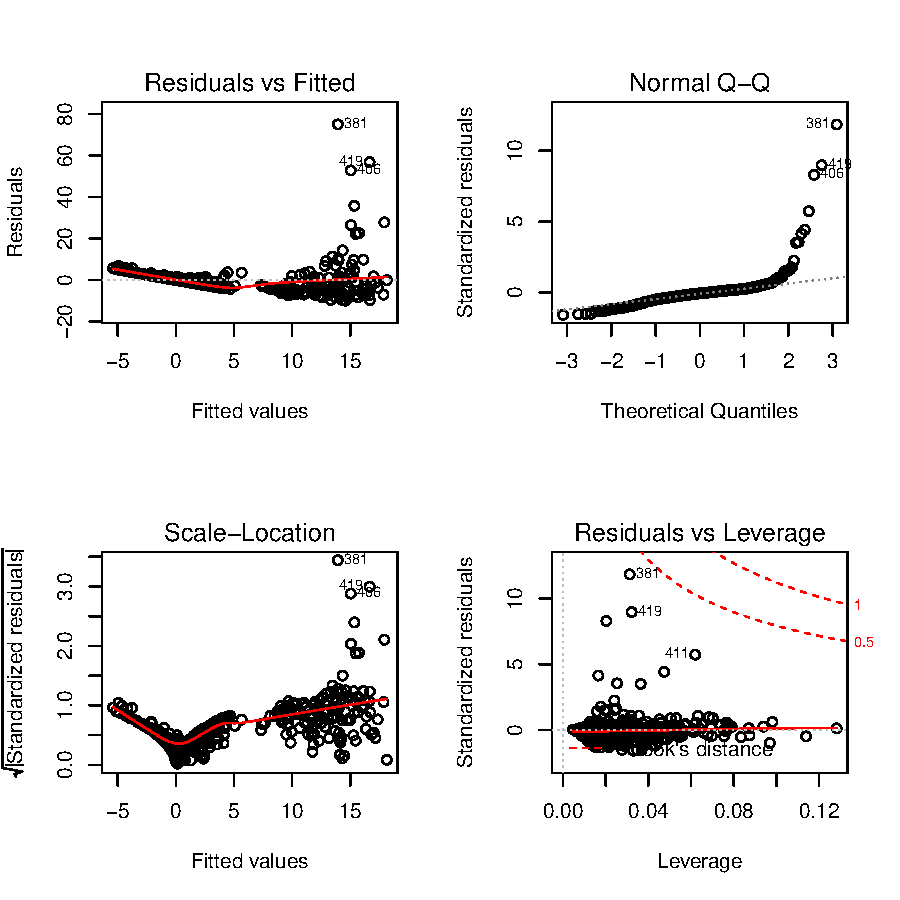
\includegraphics{mutivariblelm-15b}
\begin{enumerate}
{\color{red}
\item For predicators zn, dis, rad, black, lstat, medv we can reject null hypothesis.
}
\end{enumerate}

\part{c}
\begin{Schunk}
\begin{Sinput}
> univari.coef = c(coef(fit.zn)[2],
+                  coef(fit.indus)[2],
+                  coef(fit.chas)[2],
+                  coef(fit.nox)[2],
+                  coef(fit.rm)[2],
+                  coef(fit.age)[2],
+                  coef(fit.dis)[2],
+                  coef(fit.rad)[2],
+                  coef(fit.tax)[2],
+                  coef(fit.ptratio)[2],
+                  coef(fit.black)[2],
+                  coef(fit.lstat)[2],
+                  coef(fit.medv)[2])
> allvari.coef = coef(fit.all)[-1]
> plot(allvari.coef ~ univari.coef)
\end{Sinput}
\end{Schunk}
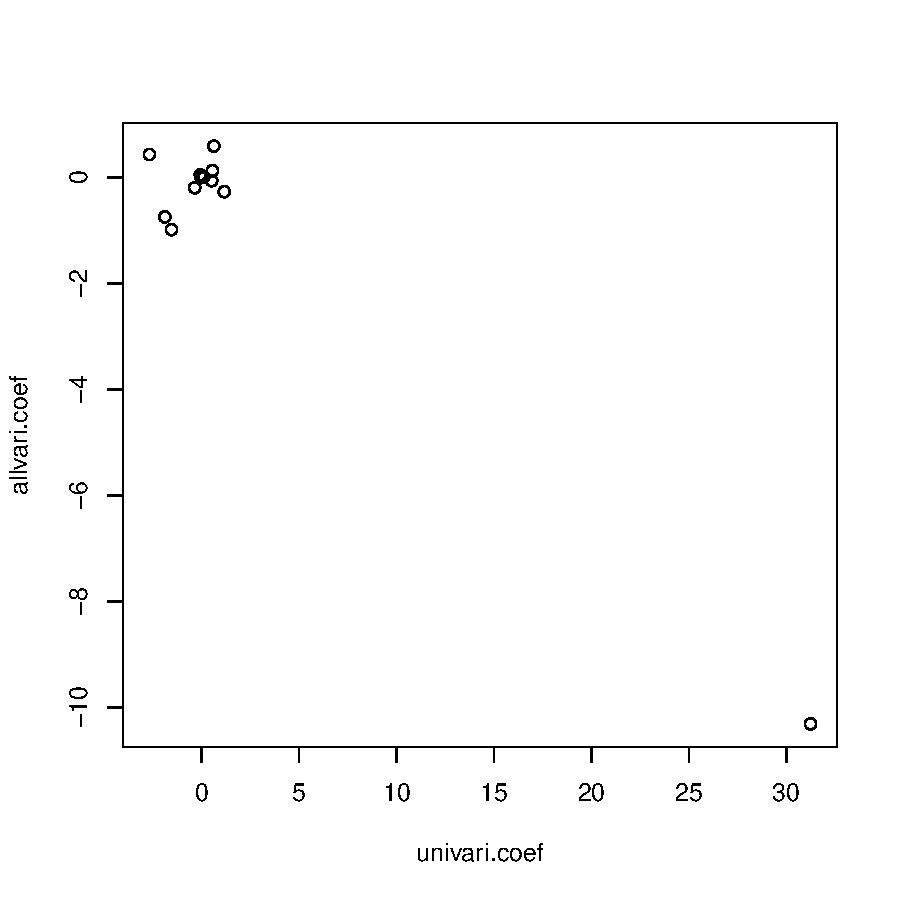
\includegraphics{mutivariblelm-15c}
\begin{enumerate}
{\color{red}
\item From the plots we can see that for most of the predictors, coefficient of univariable regression is higher than multiple regression. Some changed from positive to negative. And there is one point very interesting: the coefficient of nox is 31 in univariable regression, but changed to -10 in multiple regression.
}
\end{enumerate}


\part{d}
\begin{Schunk}
\begin{Sinput}
> fit.age = lm(crim ~ poly(age, 3))
> summary(fit.age)
\end{Sinput}
\begin{Soutput}
Call:
lm(formula = crim ~ poly(age, 3))

Residuals:
   Min     1Q Median     3Q    Max 
-9.762 -2.673 -0.516  0.019 82.842 

Coefficients:
              Estimate Std. Error t value Pr(>|t|)    
(Intercept)     3.6135     0.3485  10.368  < 2e-16 ***
poly(age, 3)1  68.1820     7.8397   8.697  < 2e-16 ***
poly(age, 3)2  37.4845     7.8397   4.781 2.29e-06 ***
poly(age, 3)3  21.3532     7.8397   2.724  0.00668 ** 
---
Signif. codes:  0 ‘***’ 0.001 ‘**’ 0.01 ‘*’ 0.05 ‘.’ 0.1 ‘ ’ 1

Residual standard error: 7.84 on 502 degrees of freedom
Multiple R-squared:  0.1742,	Adjusted R-squared:  0.1693 
F-statistic: 35.31 on 3 and 502 DF,  p-value: < 2.2e-16
\end{Soutput}
\begin{Sinput}
> par(mfrow = c(2,2))
> plot(fit.age)
\end{Sinput}
\end{Schunk}
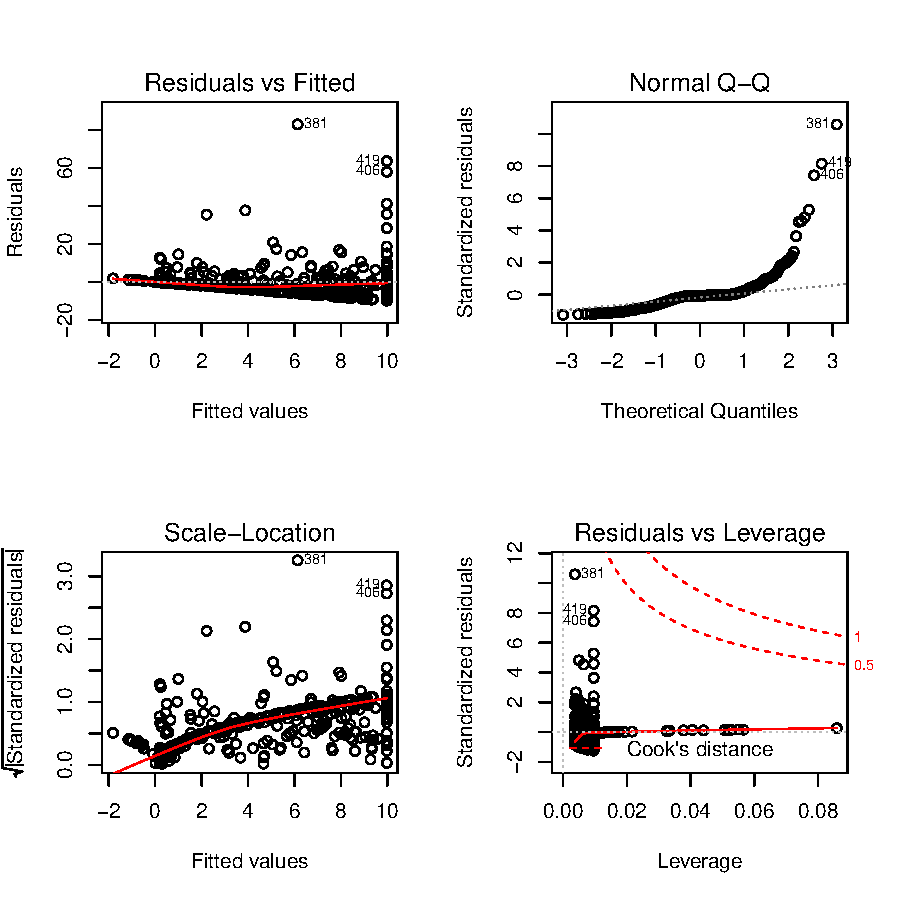
\includegraphics{mutivariblelm-age2}

\begin{Schunk}
\begin{Sinput}
> fit.black = lm(crim ~ poly(black, 3))
> summary(fit.black)
\end{Sinput}
\begin{Soutput}
Call:
lm(formula = crim ~ poly(black, 3))

Residuals:
    Min      1Q  Median      3Q     Max 
-13.096  -2.343  -2.128  -1.439  86.790 

Coefficients:
                Estimate Std. Error t value Pr(>|t|)    
(Intercept)       3.6135     0.3536  10.218   <2e-16 ***
poly(black, 3)1 -74.4312     7.9546  -9.357   <2e-16 ***
poly(black, 3)2   5.9264     7.9546   0.745    0.457    
poly(black, 3)3  -4.8346     7.9546  -0.608    0.544    
---
Signif. codes:  0 ‘***’ 0.001 ‘**’ 0.01 ‘*’ 0.05 ‘.’ 0.1 ‘ ’ 1

Residual standard error: 7.955 on 502 degrees of freedom
Multiple R-squared:  0.1498,	Adjusted R-squared:  0.1448 
F-statistic: 29.49 on 3 and 502 DF,  p-value: < 2.2e-16
\end{Soutput}
\begin{Sinput}
> par(mfrow = c(2,2))
> plot(fit.black)
\end{Sinput}
\end{Schunk}
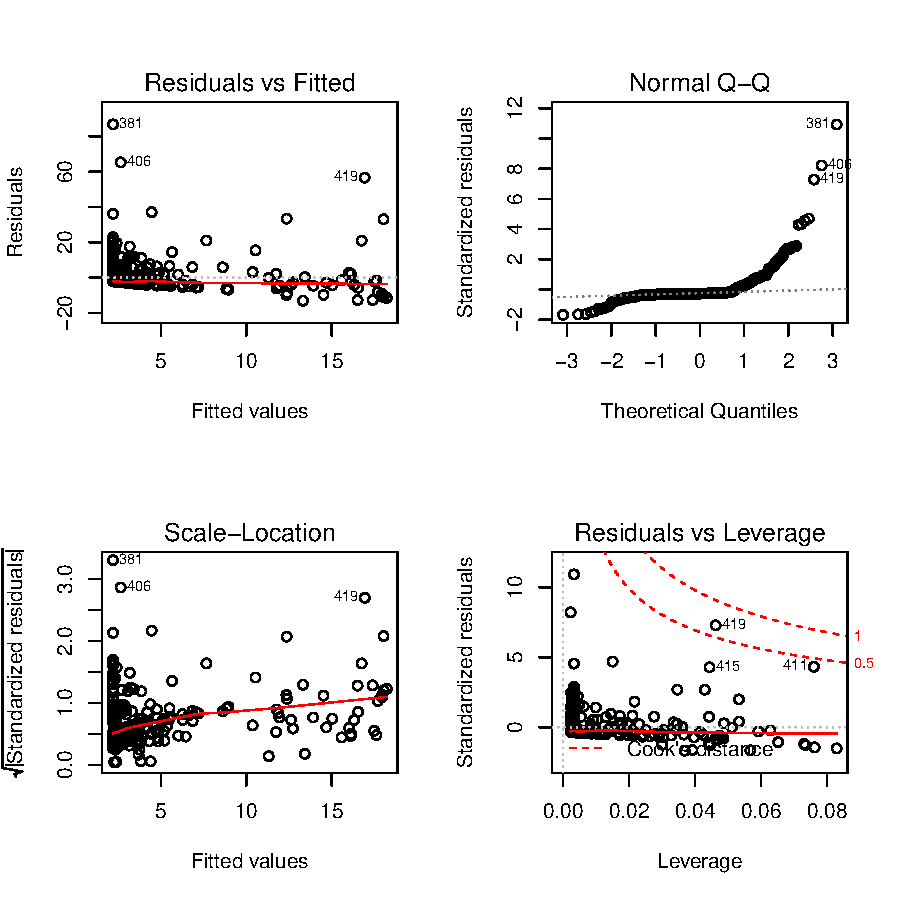
\includegraphics{mutivariblelm-black2}

\begin{Schunk}
\begin{Sinput}
> fit.dis = lm(crim ~ poly(dis, 3))
> summary(fit.dis)
\end{Sinput}
\begin{Soutput}
Call:
lm(formula = crim ~ poly(dis, 3))

Residuals:
    Min      1Q  Median      3Q     Max 
-10.757  -2.588   0.031   1.267  76.378 

Coefficients:
              Estimate Std. Error t value Pr(>|t|)    
(Intercept)     3.6135     0.3259  11.087  < 2e-16 ***
poly(dis, 3)1 -73.3886     7.3315 -10.010  < 2e-16 ***
poly(dis, 3)2  56.3730     7.3315   7.689 7.87e-14 ***
poly(dis, 3)3 -42.6219     7.3315  -5.814 1.09e-08 ***
---
Signif. codes:  0 ‘***’ 0.001 ‘**’ 0.01 ‘*’ 0.05 ‘.’ 0.1 ‘ ’ 1

Residual standard error: 7.331 on 502 degrees of freedom
Multiple R-squared:  0.2778,	Adjusted R-squared:  0.2735 
F-statistic: 64.37 on 3 and 502 DF,  p-value: < 2.2e-16
\end{Soutput}
\begin{Sinput}
> par(mfrow = c(2,2))
> plot(fit.dis)
\end{Sinput}
\end{Schunk}
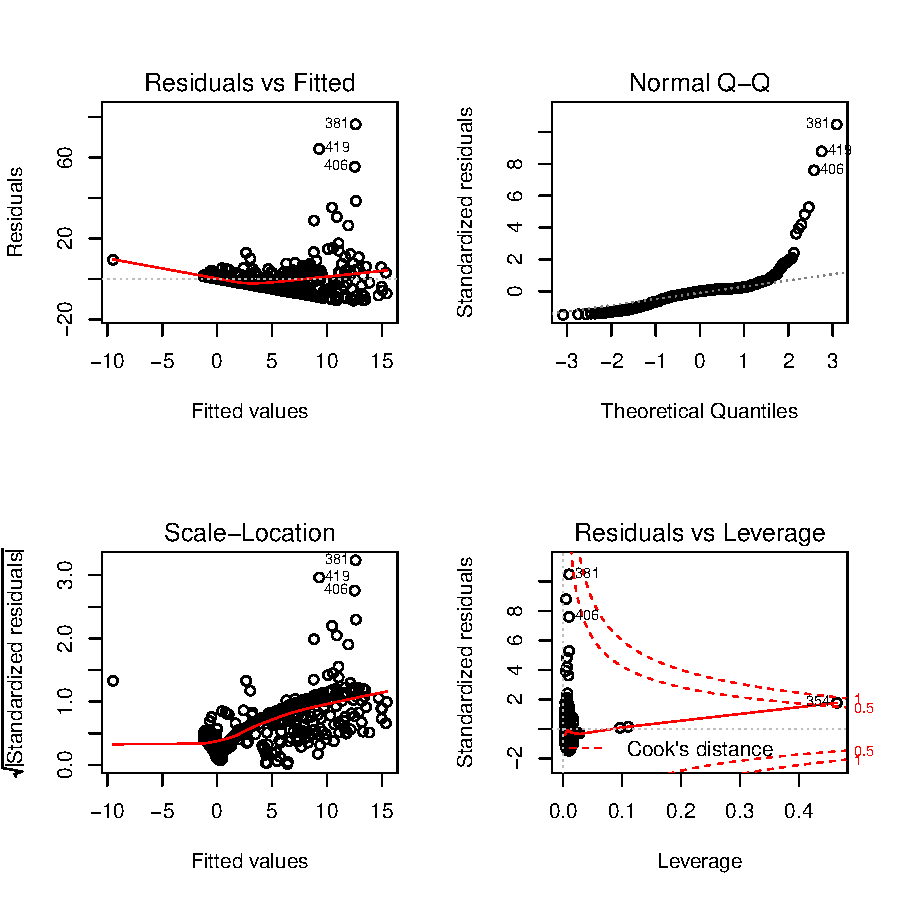
\includegraphics{mutivariblelm-dis2}

\begin{Schunk}
\begin{Sinput}
> fit.indus = lm(crim ~ poly(indus, 3))
> summary(fit.indus)
\end{Sinput}
\begin{Soutput}
Call:
lm(formula = crim ~ poly(indus, 3))

Residuals:
   Min     1Q Median     3Q    Max 
-8.278 -2.514  0.054  0.764 79.713 

Coefficients:
                Estimate Std. Error t value Pr(>|t|)    
(Intercept)        3.614      0.330  10.950  < 2e-16 ***
poly(indus, 3)1   78.591      7.423  10.587  < 2e-16 ***
poly(indus, 3)2  -24.395      7.423  -3.286  0.00109 ** 
poly(indus, 3)3  -54.130      7.423  -7.292  1.2e-12 ***
---
Signif. codes:  0 ‘***’ 0.001 ‘**’ 0.01 ‘*’ 0.05 ‘.’ 0.1 ‘ ’ 1

Residual standard error: 7.423 on 502 degrees of freedom
Multiple R-squared:  0.2597,	Adjusted R-squared:  0.2552 
F-statistic: 58.69 on 3 and 502 DF,  p-value: < 2.2e-16
\end{Soutput}
\begin{Sinput}
> par(mfrow = c(2,2))
> plot(fit.indus)
\end{Sinput}
\end{Schunk}
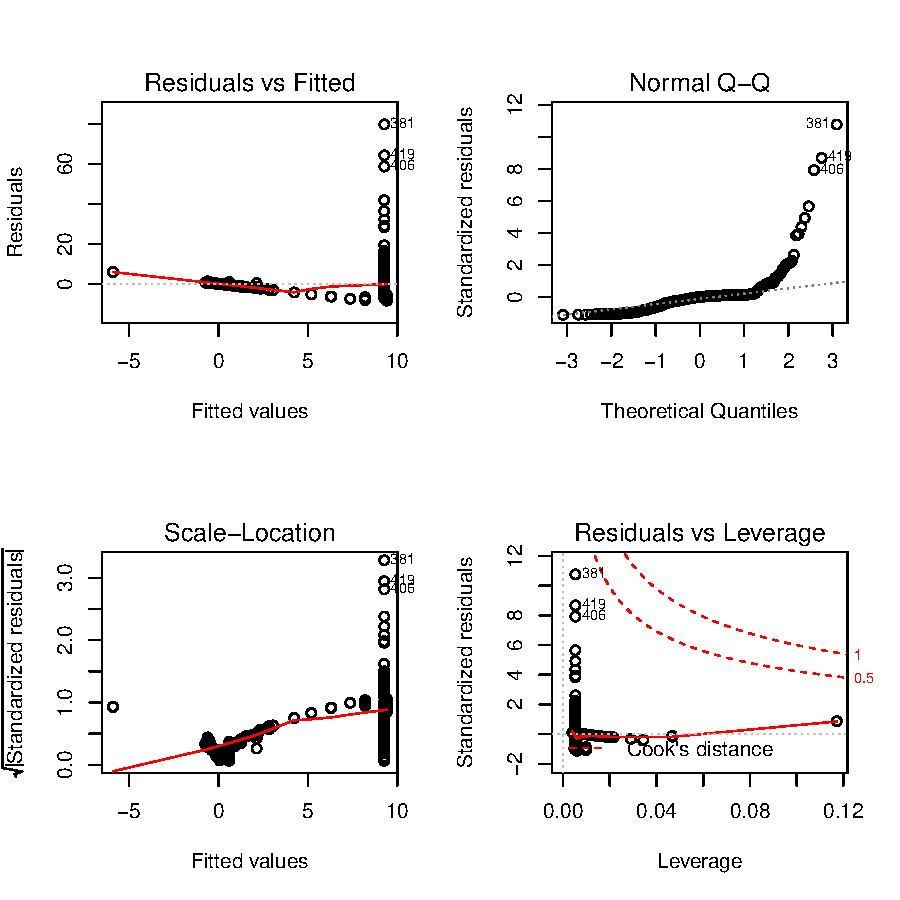
\includegraphics{mutivariblelm-indus2}

\begin{Schunk}
\begin{Sinput}
> fit.lstat = lm(crim ~ poly(lstat, 3))
> summary(fit.lstat)
\end{Sinput}
\begin{Soutput}
Call:
lm(formula = crim ~ poly(lstat, 3))

Residuals:
    Min      1Q  Median      3Q     Max 
-15.234  -2.151  -0.486   0.066  83.353 

Coefficients:
                Estimate Std. Error t value Pr(>|t|)    
(Intercept)       3.6135     0.3392  10.654   <2e-16 ***
poly(lstat, 3)1  88.0697     7.6294  11.543   <2e-16 ***
poly(lstat, 3)2  15.8882     7.6294   2.082   0.0378 *  
poly(lstat, 3)3 -11.5740     7.6294  -1.517   0.1299    
---
Signif. codes:  0 ‘***’ 0.001 ‘**’ 0.01 ‘*’ 0.05 ‘.’ 0.1 ‘ ’ 1

Residual standard error: 7.629 on 502 degrees of freedom
Multiple R-squared:  0.2179,	Adjusted R-squared:  0.2133 
F-statistic: 46.63 on 3 and 502 DF,  p-value: < 2.2e-16
\end{Soutput}
\begin{Sinput}
> par(mfrow = c(2,2))
> plot(fit.lstat)
\end{Sinput}
\end{Schunk}
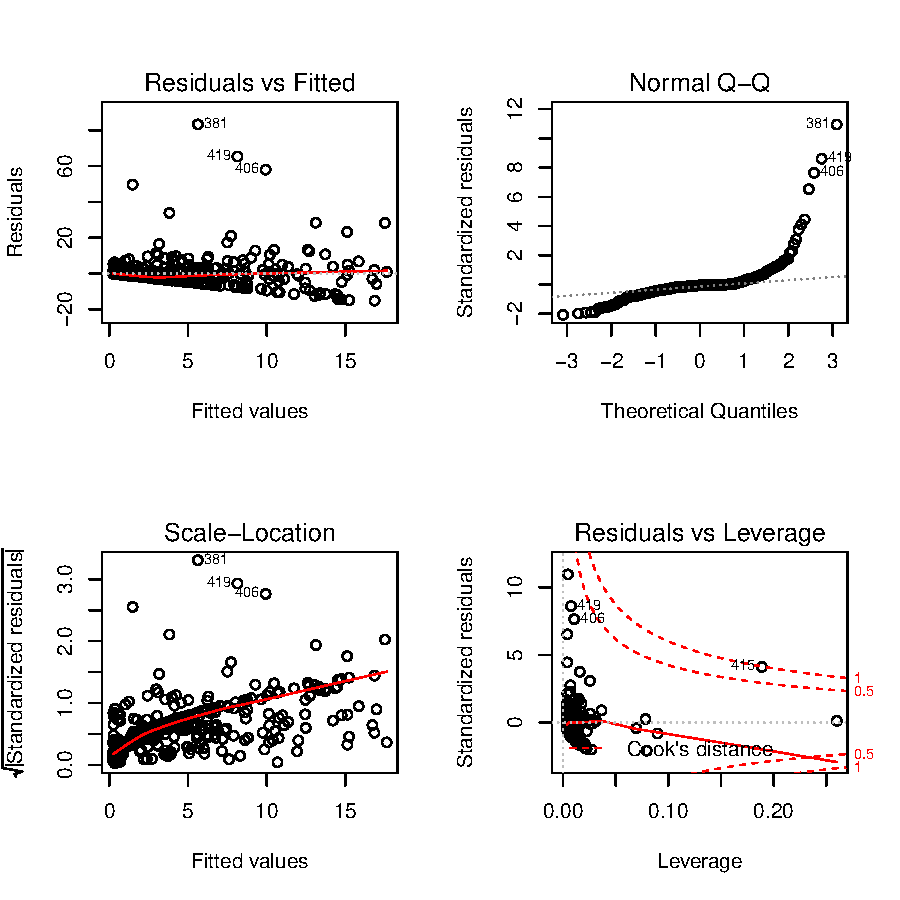
\includegraphics{mutivariblelm-lstat2}

\begin{Schunk}
\begin{Sinput}
> fit.medv = lm(crim ~ poly(medv, 3))
> summary(fit.medv)
\end{Sinput}
\begin{Soutput}
Call:
lm(formula = crim ~ poly(medv, 3))

Residuals:
    Min      1Q  Median      3Q     Max 
-24.427  -1.976  -0.437   0.439  73.655 

Coefficients:
               Estimate Std. Error t value Pr(>|t|)    
(Intercept)       3.614      0.292  12.374  < 2e-16 ***
poly(medv, 3)1  -75.058      6.569 -11.426  < 2e-16 ***
poly(medv, 3)2   88.086      6.569  13.409  < 2e-16 ***
poly(medv, 3)3  -48.033      6.569  -7.312 1.05e-12 ***
---
Signif. codes:  0 ‘***’ 0.001 ‘**’ 0.01 ‘*’ 0.05 ‘.’ 0.1 ‘ ’ 1

Residual standard error: 6.569 on 502 degrees of freedom
Multiple R-squared:  0.4202,	Adjusted R-squared:  0.4167 
F-statistic: 121.3 on 3 and 502 DF,  p-value: < 2.2e-16
\end{Soutput}
\begin{Sinput}
> par(mfrow = c(2,2))
> plot(fit.medv)
\end{Sinput}
\end{Schunk}
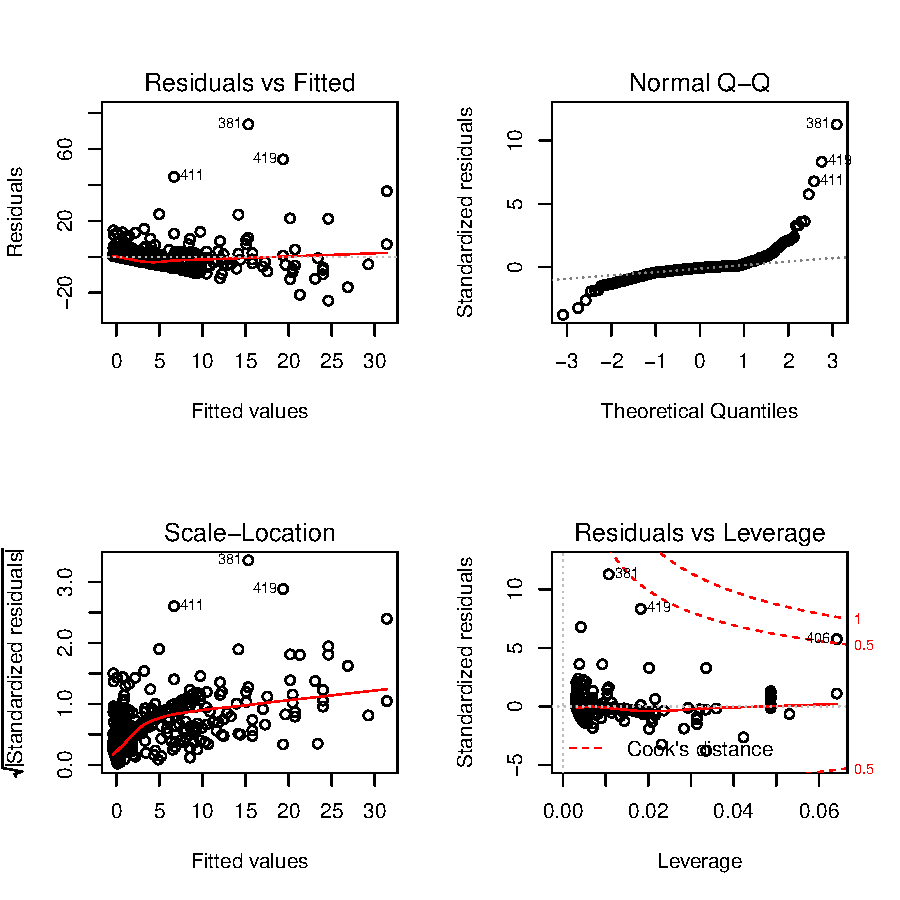
\includegraphics{mutivariblelm-medv2}

\begin{Schunk}
\begin{Sinput}
> fit.nox = lm(crim ~ poly(nox, 3))
> summary(fit.nox)
\end{Sinput}
\begin{Soutput}
Call:
lm(formula = crim ~ poly(nox, 3))

Residuals:
   Min     1Q Median     3Q    Max 
-9.110 -2.068 -0.255  0.739 78.302 

Coefficients:
              Estimate Std. Error t value Pr(>|t|)    
(Intercept)     3.6135     0.3216  11.237  < 2e-16 ***
poly(nox, 3)1  81.3720     7.2336  11.249  < 2e-16 ***
poly(nox, 3)2 -28.8286     7.2336  -3.985 7.74e-05 ***
poly(nox, 3)3 -60.3619     7.2336  -8.345 6.96e-16 ***
---
Signif. codes:  0 ‘***’ 0.001 ‘**’ 0.01 ‘*’ 0.05 ‘.’ 0.1 ‘ ’ 1

Residual standard error: 7.234 on 502 degrees of freedom
Multiple R-squared:  0.297,	Adjusted R-squared:  0.2928 
F-statistic: 70.69 on 3 and 502 DF,  p-value: < 2.2e-16
\end{Soutput}
\begin{Sinput}
> par(mfrow = c(2,2))
> plot(fit.nox)
\end{Sinput}
\end{Schunk}
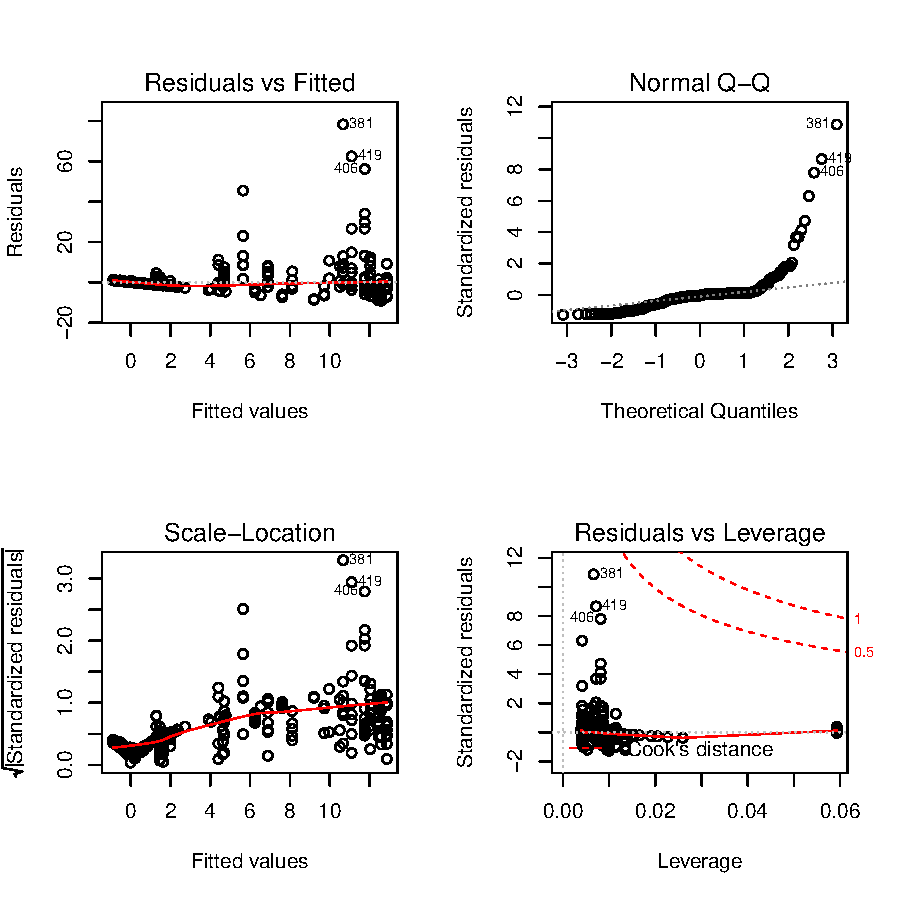
\includegraphics{mutivariblelm-nox2}

\begin{Schunk}
\begin{Sinput}
> fit.ptratio = lm(crim ~ poly(ptratio, 3))
> summary(fit.ptratio)
\end{Sinput}
\begin{Soutput}
Call:
lm(formula = crim ~ poly(ptratio, 3))

Residuals:
   Min     1Q Median     3Q    Max 
-6.833 -4.146 -1.655  1.408 82.697 

Coefficients:
                  Estimate Std. Error t value Pr(>|t|)    
(Intercept)          3.614      0.361  10.008  < 2e-16 ***
poly(ptratio, 3)1   56.045      8.122   6.901 1.57e-11 ***
poly(ptratio, 3)2   24.775      8.122   3.050  0.00241 ** 
poly(ptratio, 3)3  -22.280      8.122  -2.743  0.00630 ** 
---
Signif. codes:  0 ‘***’ 0.001 ‘**’ 0.01 ‘*’ 0.05 ‘.’ 0.1 ‘ ’ 1

Residual standard error: 8.122 on 502 degrees of freedom
Multiple R-squared:  0.1138,	Adjusted R-squared:  0.1085 
F-statistic: 21.48 on 3 and 502 DF,  p-value: 4.171e-13
\end{Soutput}
\begin{Sinput}
> par(mfrow = c(2,2))
> plot(fit.ptratio)
\end{Sinput}
\end{Schunk}
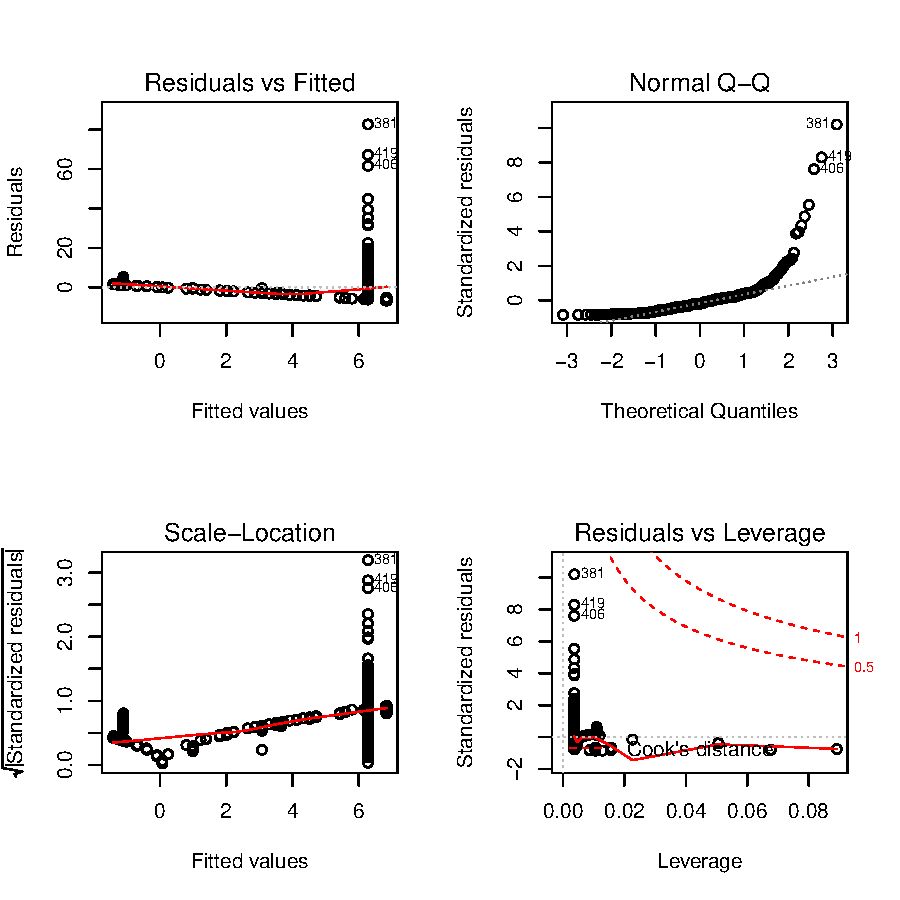
\includegraphics{mutivariblelm-ptratio2}

\begin{Schunk}
\begin{Sinput}
> fit.rad = lm(crim ~ poly(rad, 3))
> summary(fit.rad)
\end{Sinput}
\begin{Soutput}
Call:
lm(formula = crim ~ poly(rad, 3))

Residuals:
    Min      1Q  Median      3Q     Max 
-10.381  -0.412  -0.269   0.179  76.217 

Coefficients:
              Estimate Std. Error t value Pr(>|t|)    
(Intercept)     3.6135     0.2971  12.164  < 2e-16 ***
poly(rad, 3)1 120.9074     6.6824  18.093  < 2e-16 ***
poly(rad, 3)2  17.4923     6.6824   2.618  0.00912 ** 
poly(rad, 3)3   4.6985     6.6824   0.703  0.48231    
---
Signif. codes:  0 ‘***’ 0.001 ‘**’ 0.01 ‘*’ 0.05 ‘.’ 0.1 ‘ ’ 1

Residual standard error: 6.682 on 502 degrees of freedom
Multiple R-squared:    0.4,	Adjusted R-squared:  0.3965 
F-statistic: 111.6 on 3 and 502 DF,  p-value: < 2.2e-16
\end{Soutput}
\begin{Sinput}
> par(mfrow = c(2,2))
> plot(fit.rad)
\end{Sinput}
\end{Schunk}
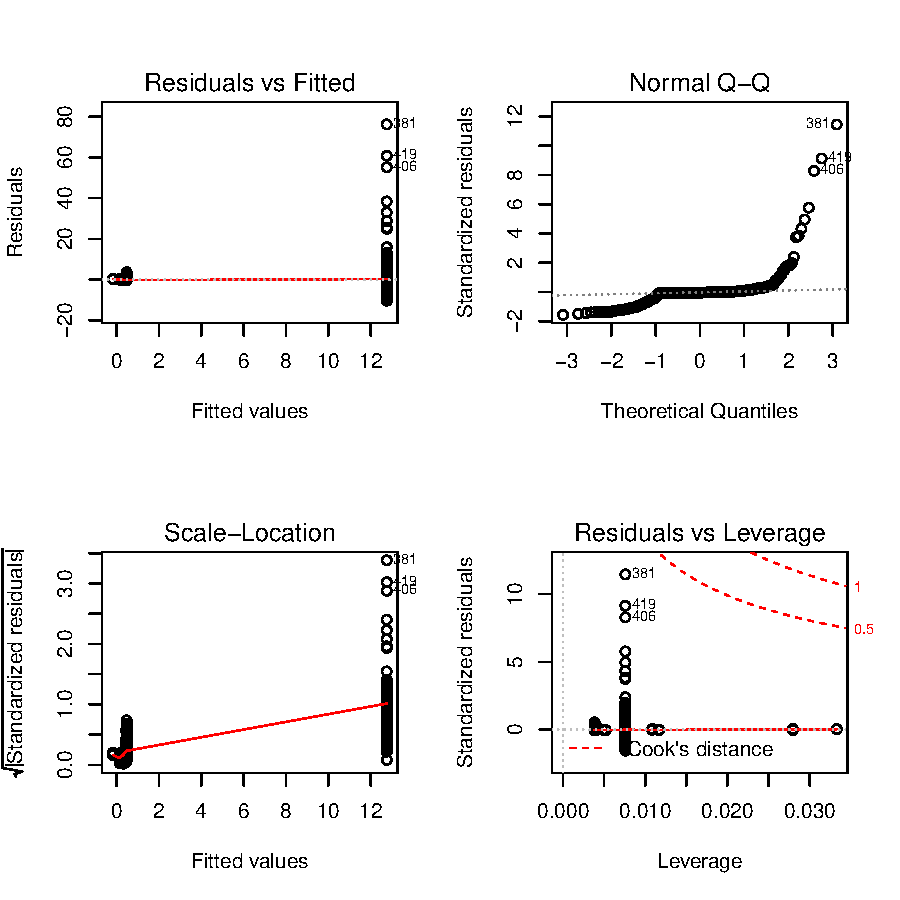
\includegraphics{mutivariblelm-rad2}

\begin{Schunk}
\begin{Sinput}
> fit.rm = lm(crim ~ poly(rm, 3))
> summary(fit.rm)
\end{Sinput}
\begin{Soutput}
Call:
lm(formula = crim ~ poly(rm, 3))

Residuals:
    Min      1Q  Median      3Q     Max 
-18.485  -3.468  -2.221  -0.015  87.219 

Coefficients:
             Estimate Std. Error t value Pr(>|t|)    
(Intercept)    3.6135     0.3703   9.758  < 2e-16 ***
poly(rm, 3)1 -42.3794     8.3297  -5.088 5.13e-07 ***
poly(rm, 3)2  26.5768     8.3297   3.191  0.00151 ** 
poly(rm, 3)3  -5.5103     8.3297  -0.662  0.50858    
---
Signif. codes:  0 ‘***’ 0.001 ‘**’ 0.01 ‘*’ 0.05 ‘.’ 0.1 ‘ ’ 1

Residual standard error: 8.33 on 502 degrees of freedom
Multiple R-squared:  0.06779,	Adjusted R-squared:  0.06222 
F-statistic: 12.17 on 3 and 502 DF,  p-value: 1.067e-07
\end{Soutput}
\begin{Sinput}
> par(mfrow = c(2,2))
> plot(fit.rm)
\end{Sinput}
\end{Schunk}
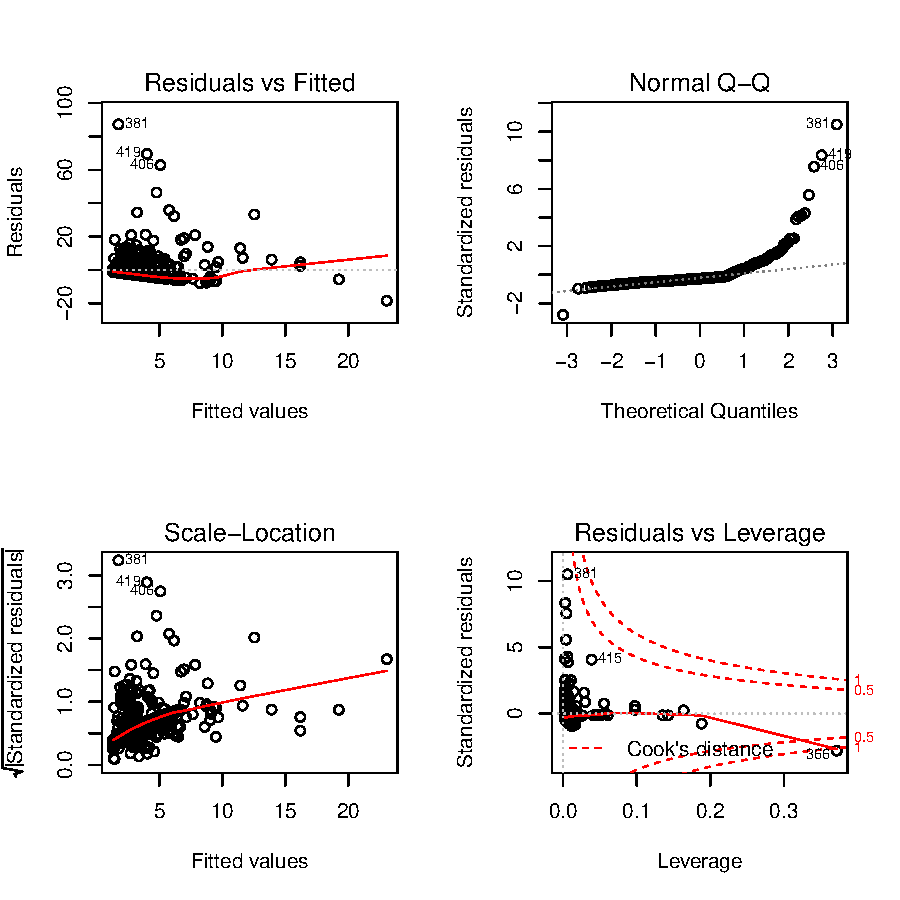
\includegraphics{mutivariblelm-rm2}

\begin{Schunk}
\begin{Sinput}
> fit.tax = lm(crim ~ poly(tax, 3))
> summary(fit.tax)
\end{Sinput}
\begin{Soutput}
Call:
lm(formula = crim ~ poly(tax, 3))

Residuals:
    Min      1Q  Median      3Q     Max 
-13.273  -1.389   0.046   0.536  76.950 

Coefficients:
              Estimate Std. Error t value Pr(>|t|)    
(Intercept)     3.6135     0.3047  11.860  < 2e-16 ***
poly(tax, 3)1 112.6458     6.8537  16.436  < 2e-16 ***
poly(tax, 3)2  32.0873     6.8537   4.682 3.67e-06 ***
poly(tax, 3)3  -7.9968     6.8537  -1.167    0.244    
---
Signif. codes:  0 ‘***’ 0.001 ‘**’ 0.01 ‘*’ 0.05 ‘.’ 0.1 ‘ ’ 1

Residual standard error: 6.854 on 502 degrees of freedom
Multiple R-squared:  0.3689,	Adjusted R-squared:  0.3651 
F-statistic:  97.8 on 3 and 502 DF,  p-value: < 2.2e-16
\end{Soutput}
\begin{Sinput}
> par(mfrow = c(2,2))
> plot(fit.tax)
\end{Sinput}
\end{Schunk}
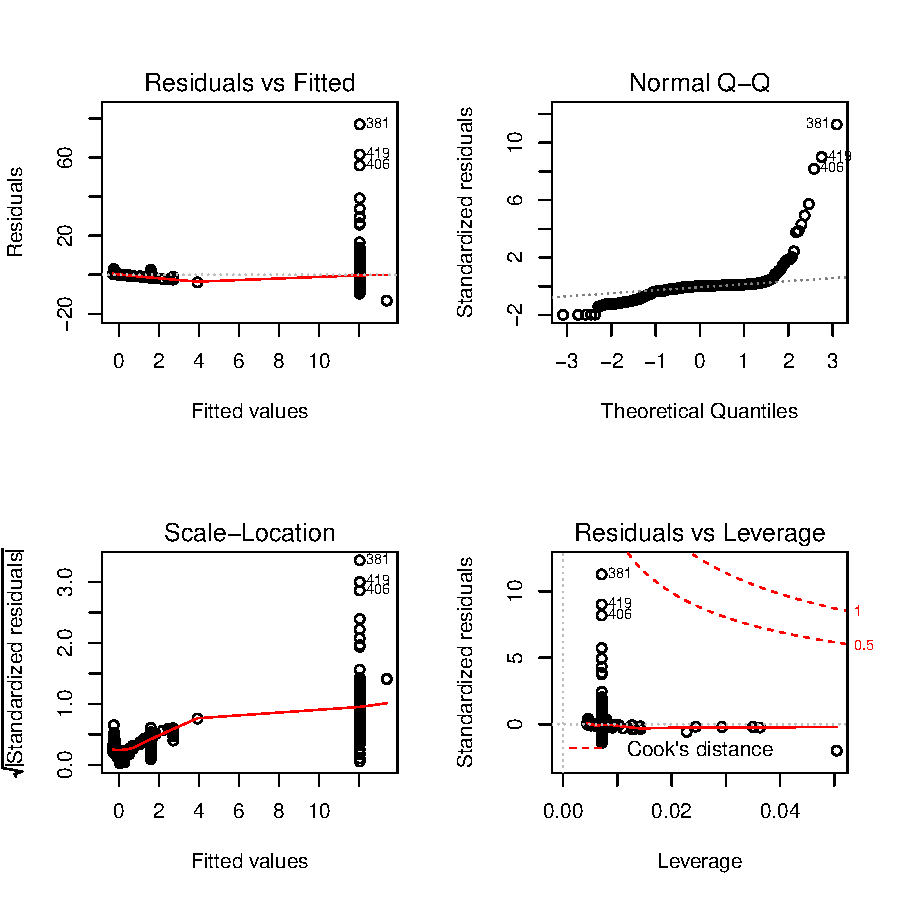
\includegraphics{mutivariblelm-tax2}

\begin{Schunk}
\begin{Sinput}
> fit.zn = lm(crim ~ poly(zn, 3))
> summary(fit.zn)
\end{Sinput}
\begin{Soutput}
Call:
lm(formula = crim ~ poly(zn, 3))

Residuals:
   Min     1Q Median     3Q    Max 
-4.821 -4.614 -1.294  0.473 84.130 

Coefficients:
             Estimate Std. Error t value Pr(>|t|)    
(Intercept)    3.6135     0.3722   9.709  < 2e-16 ***
poly(zn, 3)1 -38.7498     8.3722  -4.628  4.7e-06 ***
poly(zn, 3)2  23.9398     8.3722   2.859  0.00442 ** 
poly(zn, 3)3 -10.0719     8.3722  -1.203  0.22954    
---
Signif. codes:  0 ‘***’ 0.001 ‘**’ 0.01 ‘*’ 0.05 ‘.’ 0.1 ‘ ’ 1

Residual standard error: 8.372 on 502 degrees of freedom
Multiple R-squared:  0.05824,	Adjusted R-squared:  0.05261 
F-statistic: 10.35 on 3 and 502 DF,  p-value: 1.281e-06
\end{Soutput}
\begin{Sinput}
> par(mfrow = c(2,2))
> plot(fit.zn)
\end{Sinput}
\end{Schunk}
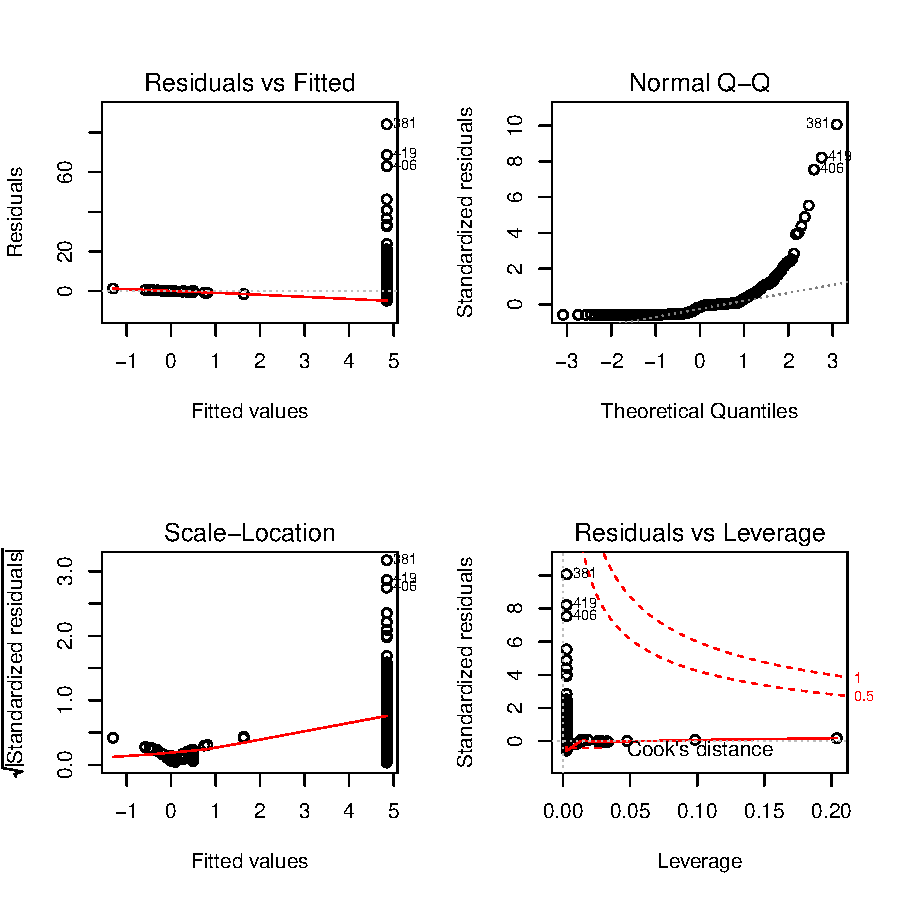
\includegraphics{mutivariblelm-zn2}
\begin{enumerate}
{\color{red}
\item There are evidence of non-linear association between all of the predictors and the response except chas and black, from the summary and plots we can see. We can see that most of the p-values of quadradic and cubic term are very small.
}
\end{enumerate}

\end{document}
